\documentclass{beamer}
%
% Choose how your presentation looks.
%
% For more themes, color themes and font themes, see:
% http://deic.uab.es/~iblanes/beamer_gallery/index_by_theme.html
%
\mode<presentation>
{
  \usetheme{default}      % or try Darmstadt, Madrid, Warsaw, ...
  \usecolortheme{default} % or try albatross, beaver, crane, ...
  \usefonttheme{default}  % or try serif, structurebold, ...
  \setbeamertemplate{navigation symbols}{}
  \setbeamertemplate{caption}[numbered]
} 

\usepackage[english]{babel}
\usepackage[utf8x]{inputenc}

\title[Your Short Title]{Version Control, Git, and GitHub}
\author{D2K Course Staff}
\institute{Rice University}
\date{February 6th, 2019}

\begin{document}

\begin{frame}
  \titlepage
\end{frame}

% Uncomment these lines for an automatically generated outline.
%\begin{frame}{Outline}
%  \tableofcontents
%\end{frame}

\section{Introduction}

\begin{frame}{Intro to Version Control}

\begin{itemize}
  \item What is version control?
  \item Why do we use version control?
  \item How will we be applying it to our projects?
\end{itemize}

\vskip 1cm

\begin{block}{Example}
Say you are building a software product, but have a lot of different ideas for potential versions, features, analyses that you want to try out. How do we manage different versions of the same product? How do we keep track of changes over time? How do we keep ourselves from descending into chaos?
\end{block}

\end{frame}

% Commands to include a figure:
%\begin{figure}
%\includegraphics[width=\textwidth]{your-figure's-file-name}
%\caption{\label{fig:your-figure}Caption goes here.}
%\end{figure}

\begin{frame}{What is Version Control?}

\begin{itemize}
  \item Version control is a system for keeping track of changes in records, files, code, etc. over time
  \item The most primitive version control method is to save different copies of your work locally with different names or timestamps every time a change is made (\textbf{BAD IDEA})
  \item How do you collaborate with other people? What if multiple people make different changes at the same time (see below)? How do you reconcile everyone's work? How do you communicate changes?
  
\end{itemize}

\begin{figure}
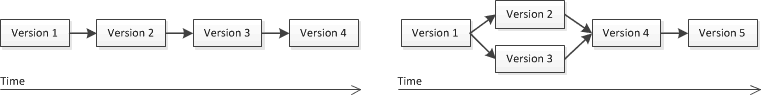
\includegraphics[width=\textwidth]{version-control-fig4.png}
\caption{\label{fig:your-figure}Versions over Time}
\end{figure}

\end{frame}

\begin{frame}{What is Version Control?}

\begin{itemize}
    \item To answer these questions, developers first created \textbf{Centralized Version Control} systems to house the codebase on a central server called a \textit{repository}
    \item These present potential problems since the code is only hosted on a single server
    \begin{itemize}
        \item More error-prone since each commit updates entire codebase
        \item Impossible to work if the single server goes down
    \end{itemize}
\end{itemize}

\begin{figure}
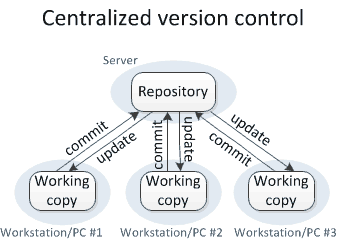
\includegraphics[width=5cm]{version-control-fig2.png}
\caption{\label{fig:your-figure}Centralized Version Control Structure}
\end{figure}
    
\end{frame}

\begin{frame}{What is Version Control?}

\begin{itemize}
    \item To address these issues and others, developers created what are known as \textbf{Distributed Version Control} systems
    \item These host the codebase or \textit{repository} across multiple servers
    \item These are advantageous to centralized systems because they
    \begin{itemize}
        \item create full backups of the repository across multiple servers/computers
        \item allow for different people to work in different ways at the same time within the same project
    \end{itemize}
\end{itemize}

\begin{figure}
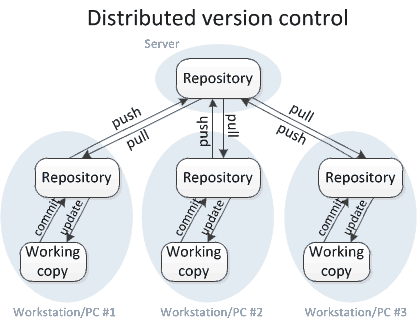
\includegraphics[width=5cm]{version-control-fig3.png}
\caption{\label{fig:your-figure}Distributed Version Control Structure}
\end{figure}
    
\end{frame}

\begin{frame}{Why do we use Version Control?}

\begin{itemize}
    \item You will need to work together!
    \item You will make mistakes!
    \item You will need to do different things at the same time!
\end{itemize}

\vskip 1cm
    
\begin{block}{Bottom Line}
Using version control systems is important and is how anyone who writes code as part of a team functions in the real world. It may be confusing at first, but it is better to deal with the initial friction than to realize you have messed up your entire codebase the night before it is due.
\end{block}

\end{frame}

\begin{frame}{How will we be applying it to our projects?}

\begin{figure}
\centering
\begin{subfigure}{\textwidth}
  \centering
  
\includegraphics[width=.45\linewidth]{logo@2x.png}
\end{subfigure}%
\begin{subfigure}{\textwidth}
  \centering
  
\includegraphics[width=.45\linewidth]{github_logo.png}
\end{subfigure}
\end{figure}

\begin{block}{}
For your teams this semester, you will be using a code hosting platform called GitHub. GitHub is a free version control tool that is based on the distributed version control system Git. GitHub allows you to track your progress and collaborate on projects from anywhere.
\end{block} 
\end{frame}

\begin{frame}{How to use GitHub}
\begin{itemize}
    \item Step 1: Create your repository (i.e. codebase)
    \item Step 2: Clone your repository to your local computer
    \item Step 3: Create a branch
    \item Step 4: Make and commit changes to your branch
    \item Step 5: Open a pull request
    \item Step 6: Merge your pull request
\end{itemize}
\begin{figure}
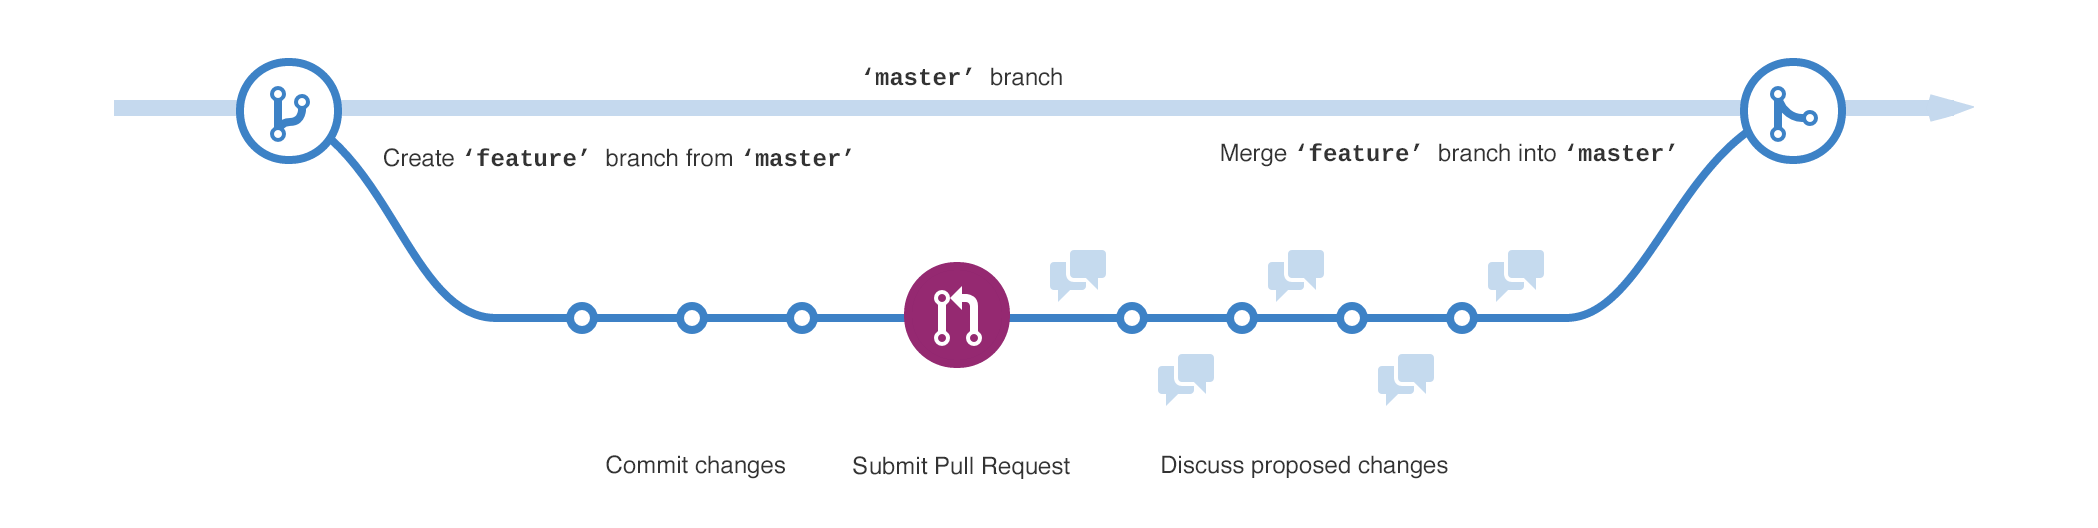
\includegraphics[width=10cm]{branching.png}
\caption{\label{fig:your-figure}GitHub Workflow}
\end{figure}
\end{frame}

\begin{frame}{Step 1: Create your repository}
\begin{itemize}
    \item Create a new repository on github.com by clicking on the + sign in the top right corner of your screen and selecting \textbf{New repository}
    \item Select \textbf{Private} repository (This is important!)
    \item Name your repository, write a short description, and initialize your repository with a README.md file before clicking \textbf{Create repository}
\begin{figure}
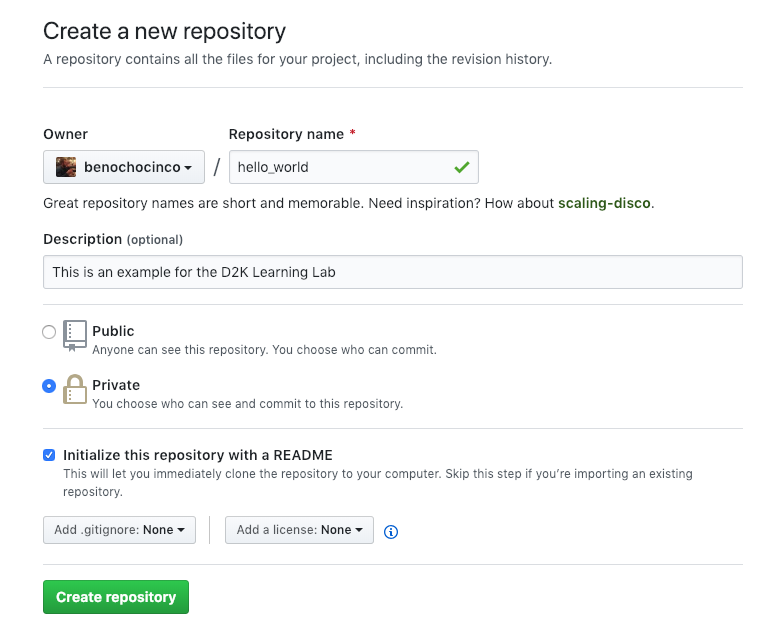
\includegraphics[width=5cm]{create_repo.png}
\end{figure}
\end{itemize}
\end{frame}

\begin{frame}{Step 2: Clone your repository}
\begin{itemize}
    \item Open GitHub desktop and click the top right corner where it says ``Current Repository", click ``Add", and then select ``Clone Repository"
    \item Copy the github.com/user/repository URL as the Repository URL and select the local path you would like to use (where you want your repository to live on your local computer)
\end{itemize}
\begin{figure}
\centering
\begin{subfigure}{\textwidth}
  \centering
  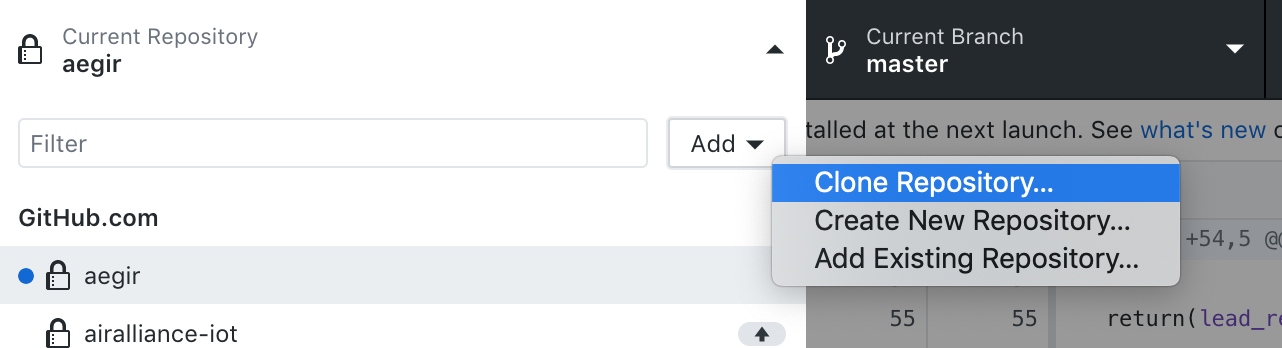
\includegraphics[width=.35\linewidth]{add_repo.png}
\end{subfigure}%
\hspace{1cm}
\begin{subfigure}{\textwidth}
  \centering
  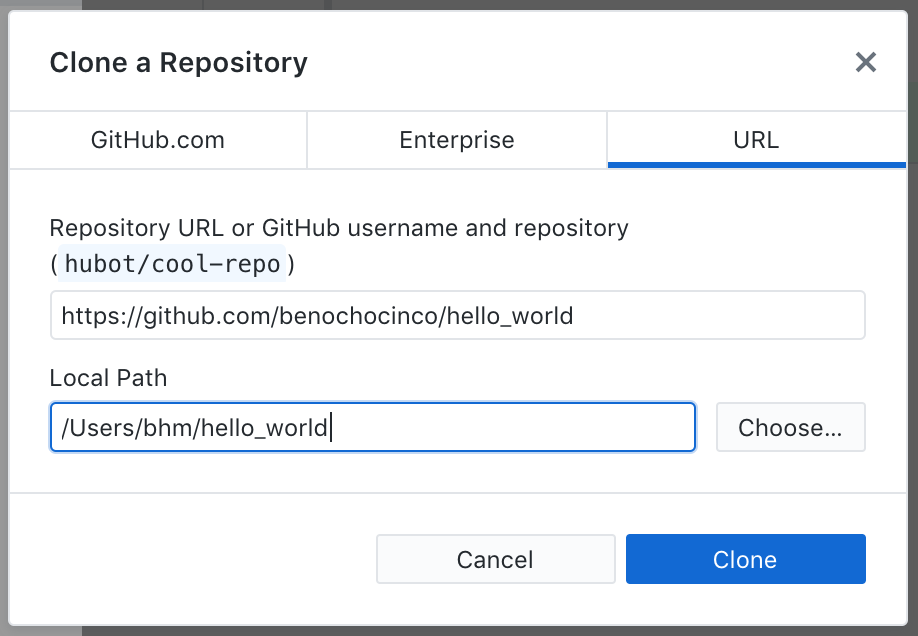
\includegraphics[width=.35\linewidth]{clone_repo.png}
\end{subfigure}
\end{figure}
\text{\textbf{Note}: you can use the command line if you prefer, but not required}
\end{frame}

\begin{frame}{Step 3: Create a branch}
\begin{itemize}
    \item Whenever you decide to start a new task or write new code you should create a \text{new} branch
    \item It is best practice to always start a new branch based on the master branch so that you are not building on top of outdated code
    \item The work you do on a branch will exist separately from the master branch until you \textit{commit}, \textit{push}, \textit{pull} and \textit{merge} (more on that later)
\end{itemize}
\begin{figure}
\centering
\begin{subfigure}{\textwidth}
  \centering
  \includegraphics[width=.35\linewidth]{create_new_branch.png}
\end{subfigure}%
\hspace{1cm}
\begin{subfigure}{\textwidth}
  \centering
  \includegraphics[width=.35\linewidth]{create_new_branch2.png}
\end{subfigure}
\end{figure}
\end{frame}

\begin{frame}{Step 4: Make and commit changes to your branch}
\begin{itemize}
    \item Any change made in your local repository will be reflected in the GitHub Desktop interface
    \item Changes can be new files or additional lines of code added to old files
\end{itemize}
\begin{figure}
\centering
\begin{subfigure}{\textwidth}
  \centering
  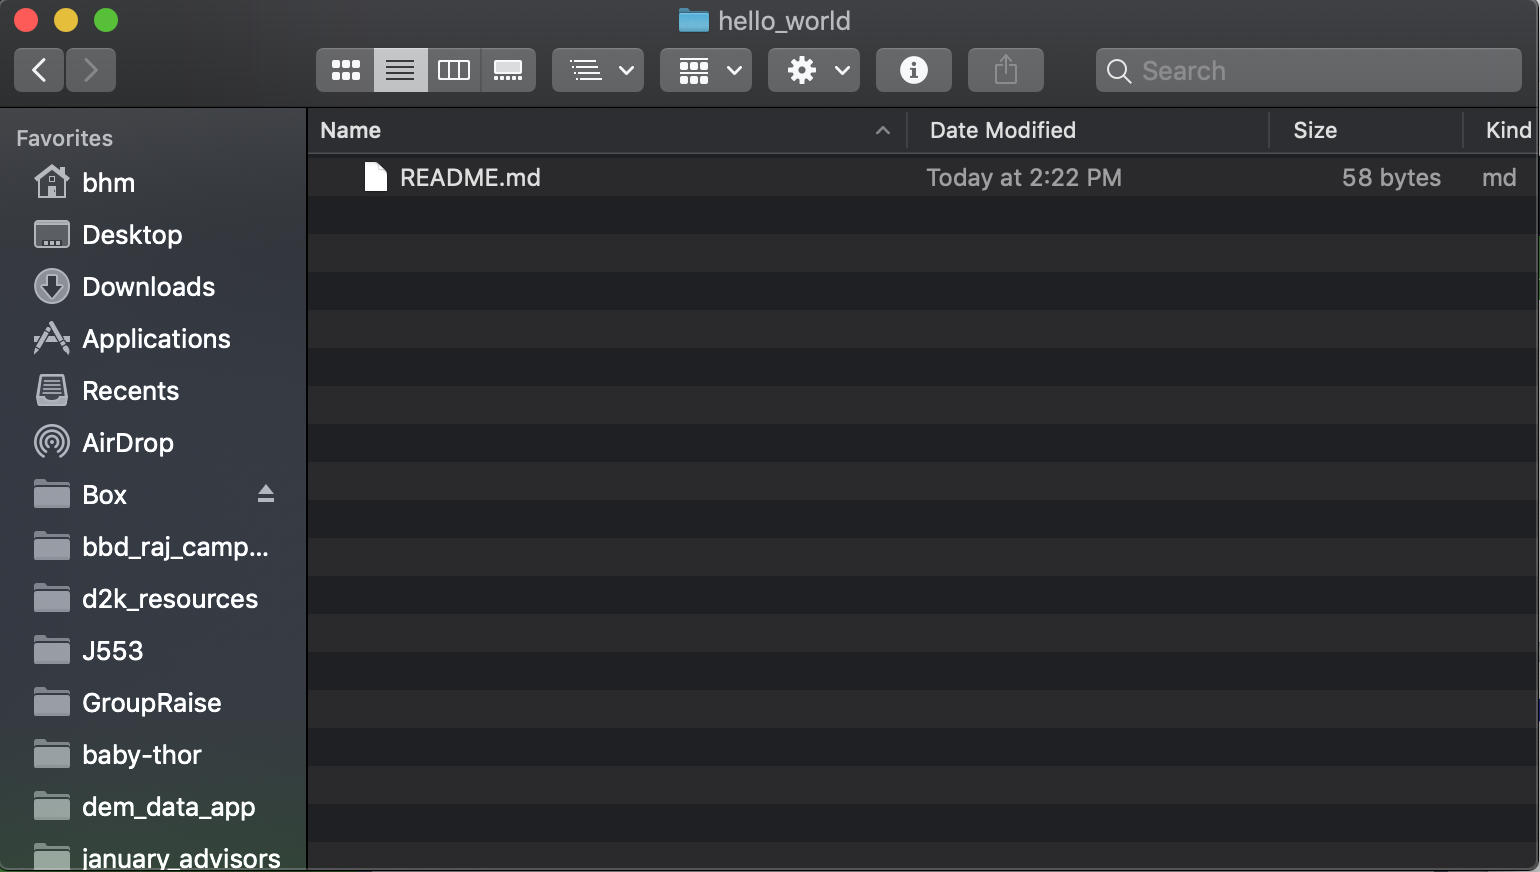
\includegraphics[width=.35\linewidth]{before_change.png}
\end{subfigure}%
\begin{subfigure}{\textwidth}
  \centering
  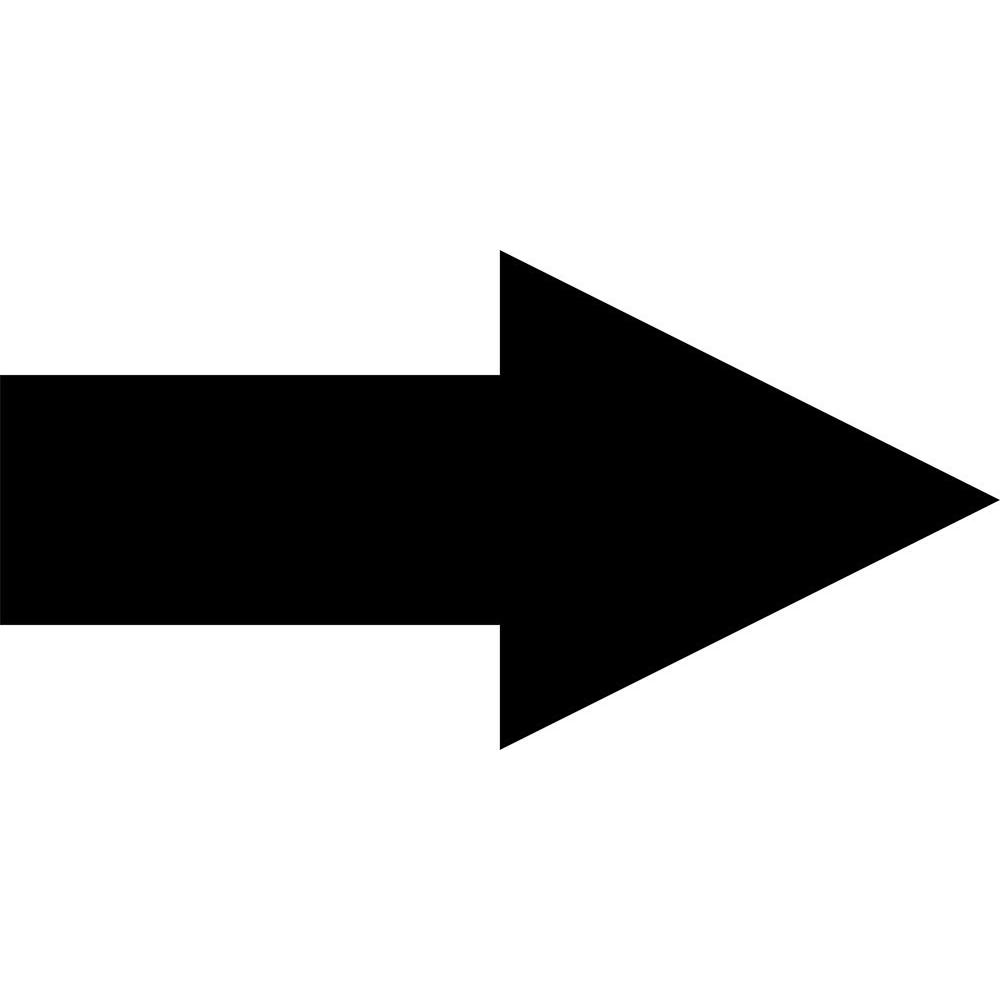
\includegraphics[width=.1\linewidth]{arrow.png}
\end{subfigure}
\begin{subfigure}{\textwidth}
  \centering
  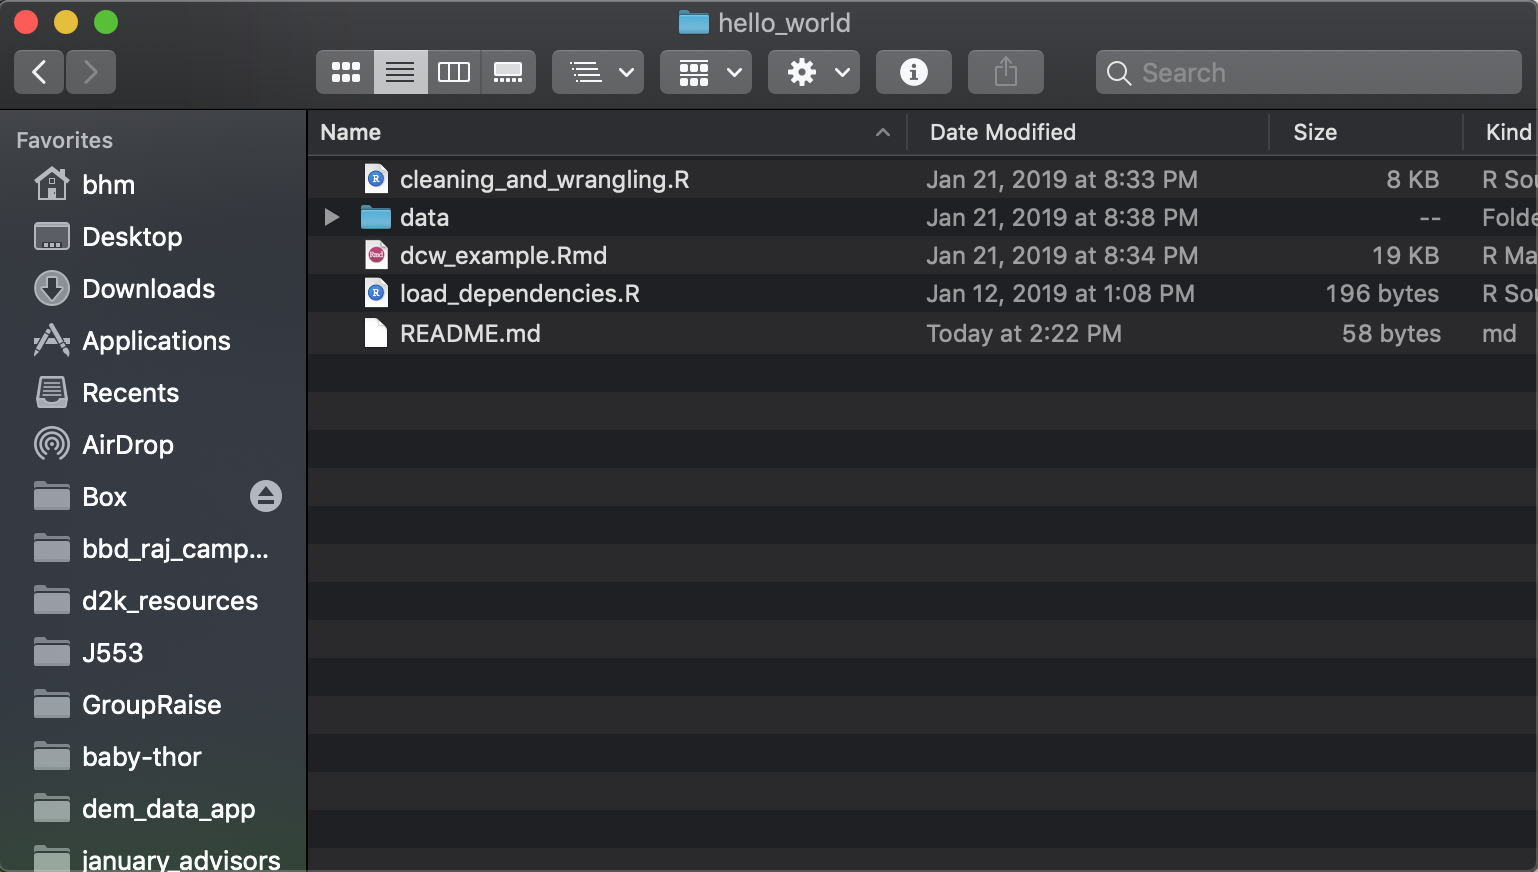
\includegraphics[width=.35\linewidth]{after_change.png}
\end{subfigure}
\end{figure}
\begin{figure}
\centering
\begin{subfigure}{\textwidth}
  \centering
  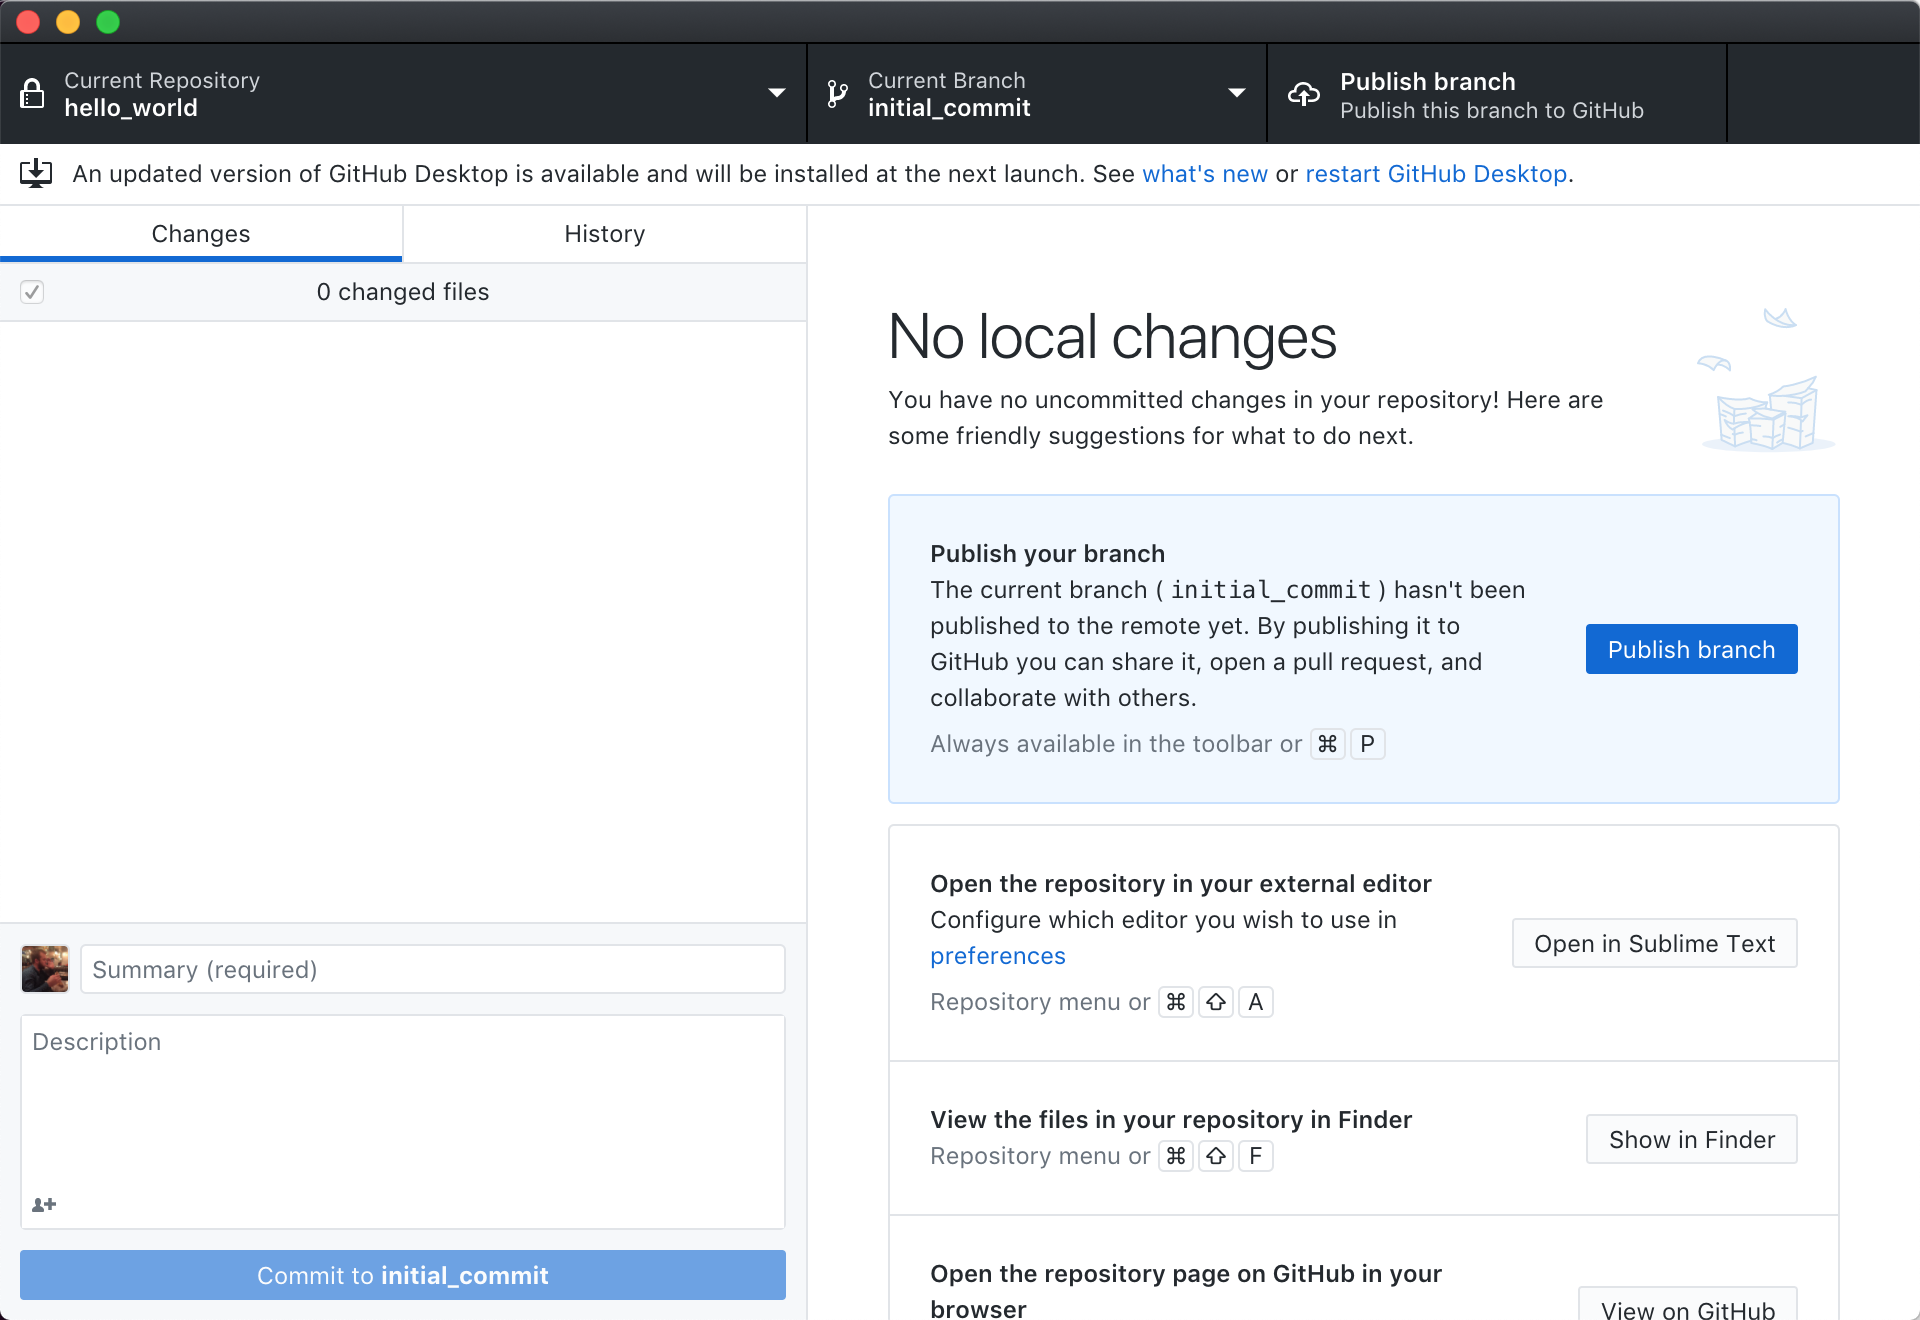
\includegraphics[width=.35\linewidth]{before_change_desktop.png}
\end{subfigure}%
\begin{subfigure}{\textwidth}
  \centering
  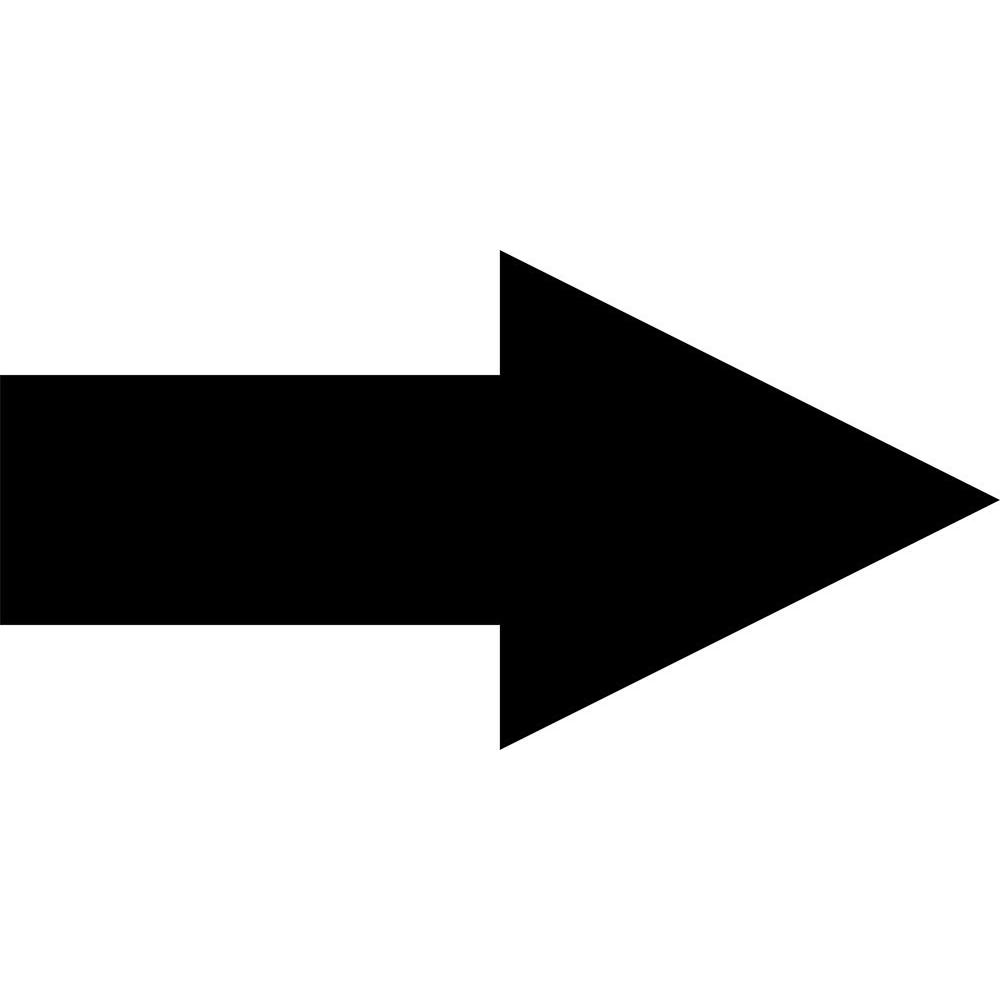
\includegraphics[width=.1\linewidth]{arrow.png}
\end{subfigure}
\begin{subfigure}{\textwidth}
  \centering
  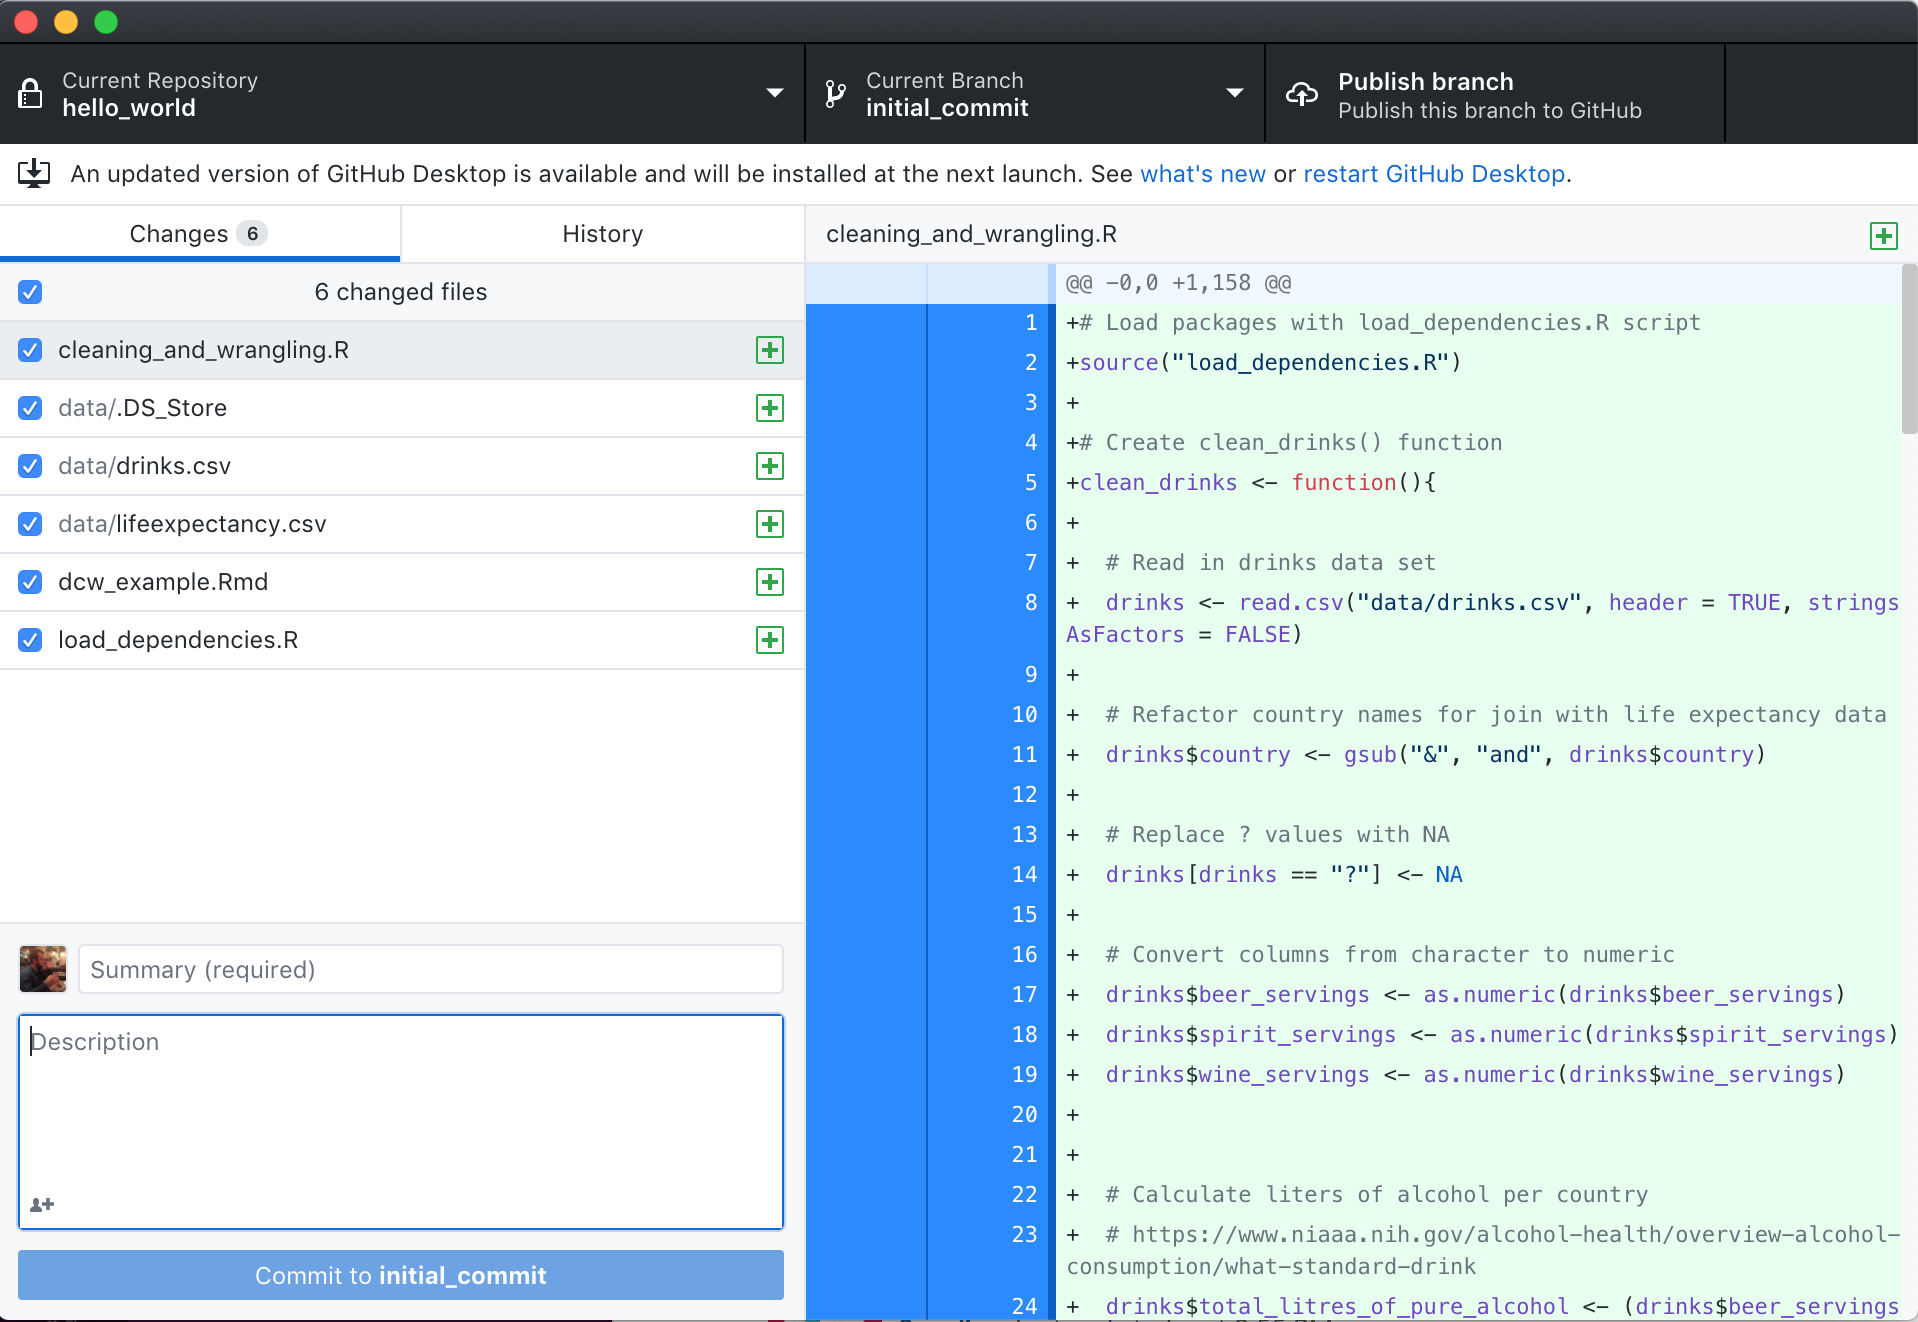
\includegraphics[width=.35\linewidth]{after_change_desktop.png}
\end{subfigure}
\end{figure}
\end{frame}

\begin{frame}{Step 4: Make and commit changes to your branch}
\begin{itemize}
    \item Once you have made a change you are happy with, commit the change to ``save" your progress locally
    \item Once you have complete your modularized task, you push your work to origin (the first push of a branch "publishes" it)
    \item After pushing your work, it is saved to the central repository on the GitHub website
\end{itemize}
\begin{figure}
\centering
\begin{subfigure}{\textwidth}
  \centering
  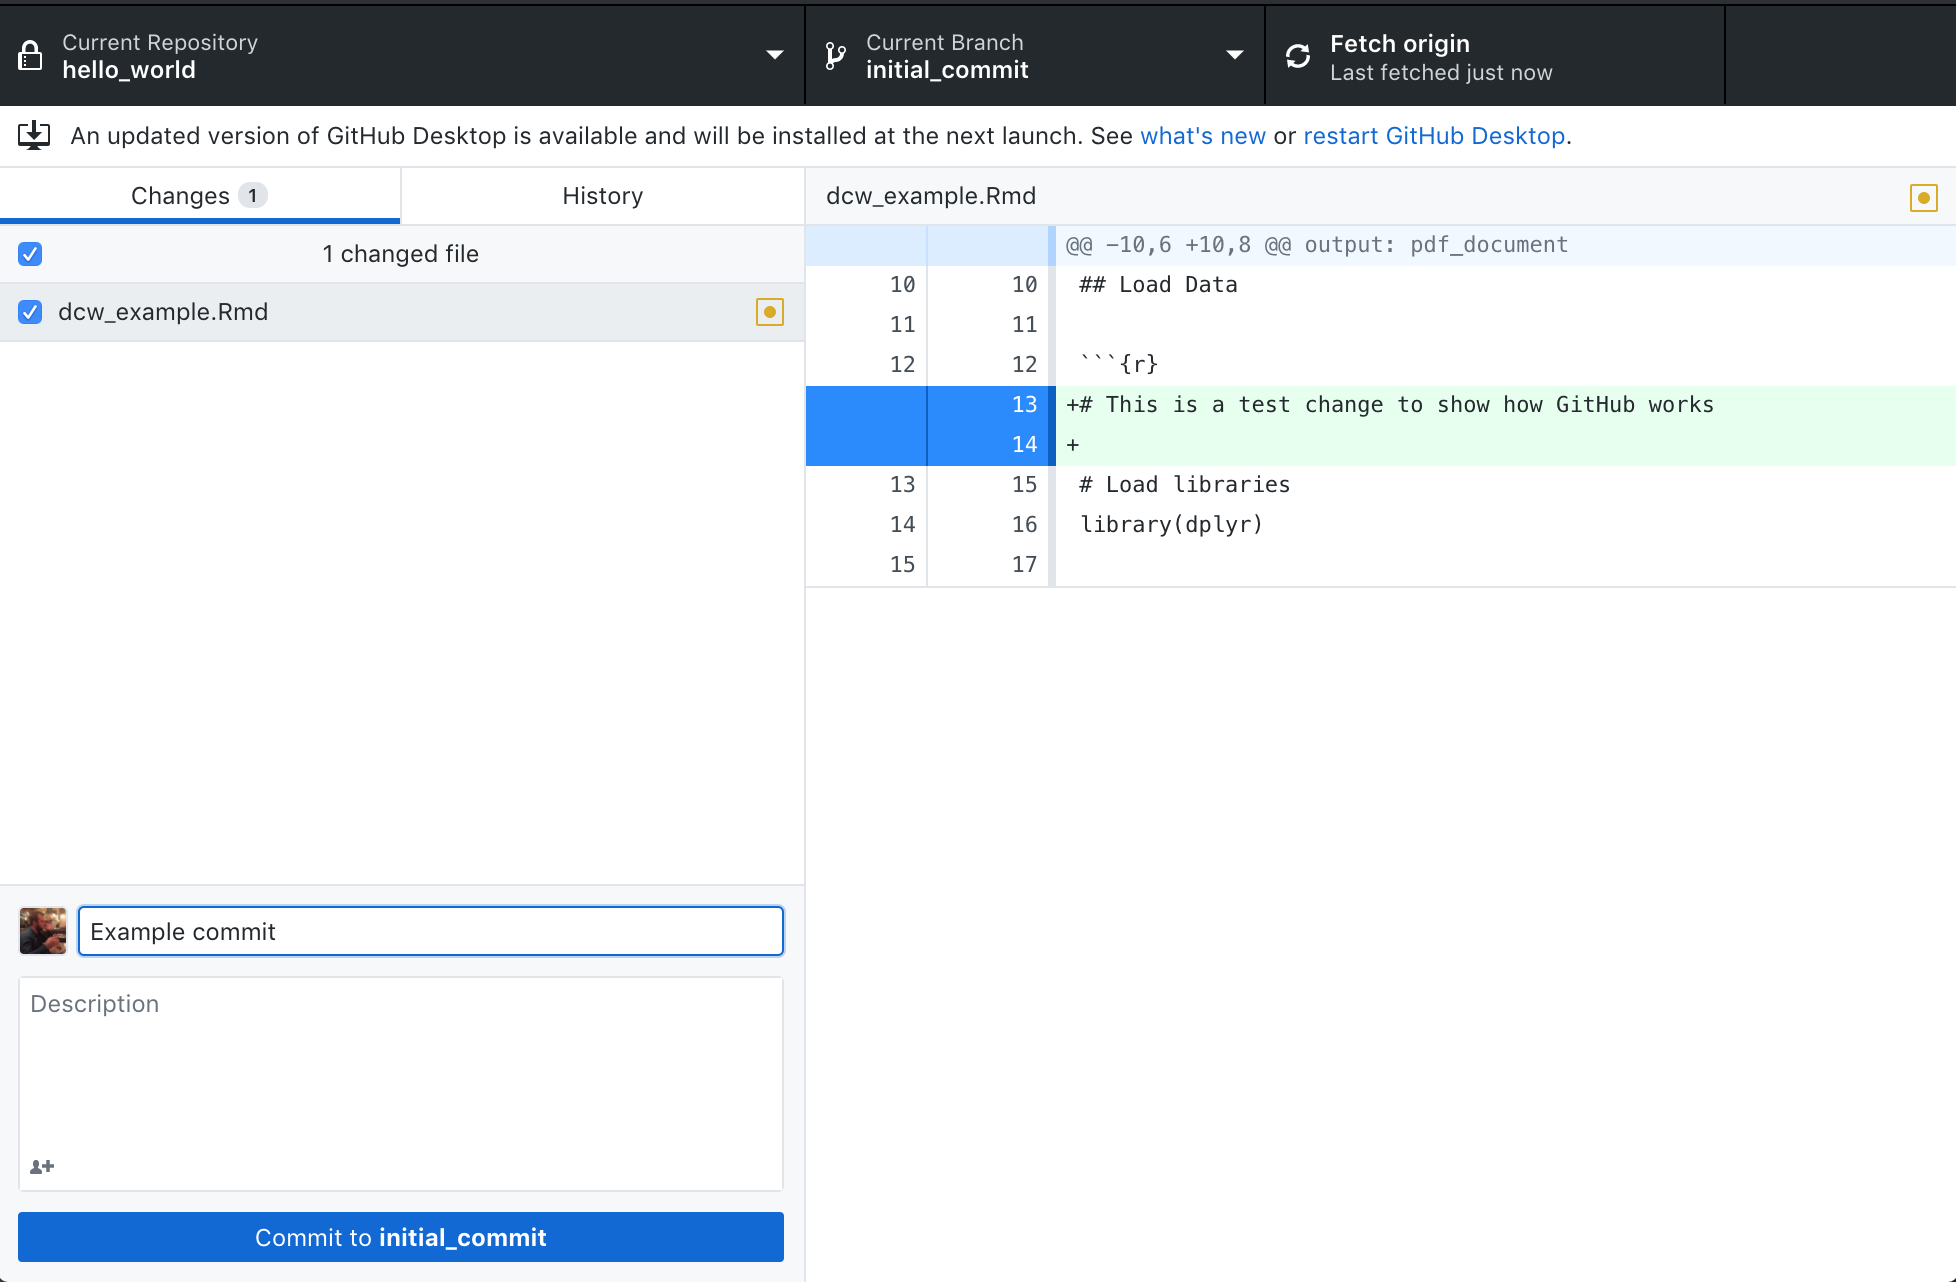
\includegraphics[width=.4\linewidth]{commit.png}
\end{subfigure}%
\begin{subfigure}{\textwidth}
  \centering
  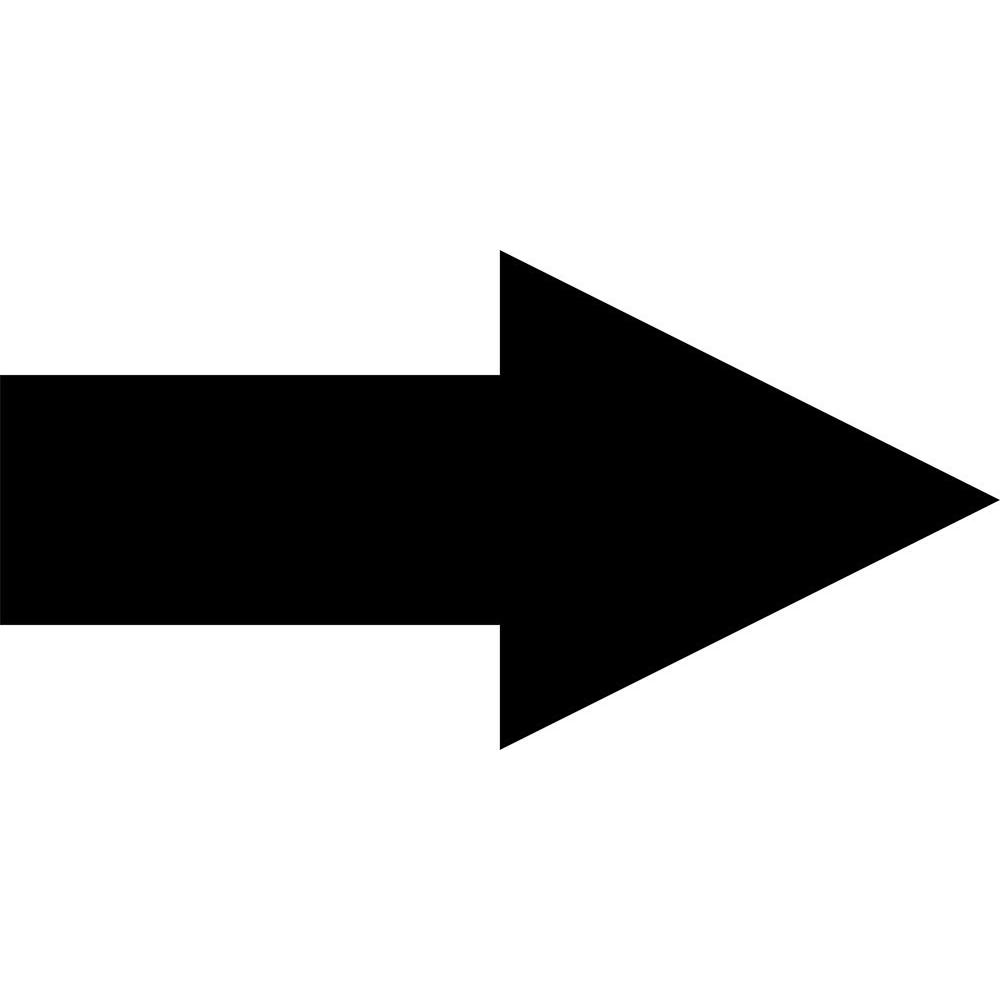
\includegraphics[width=.1\linewidth]{arrow.png}
\end{subfigure}
\begin{subfigure}{\textwidth}
  \centering
  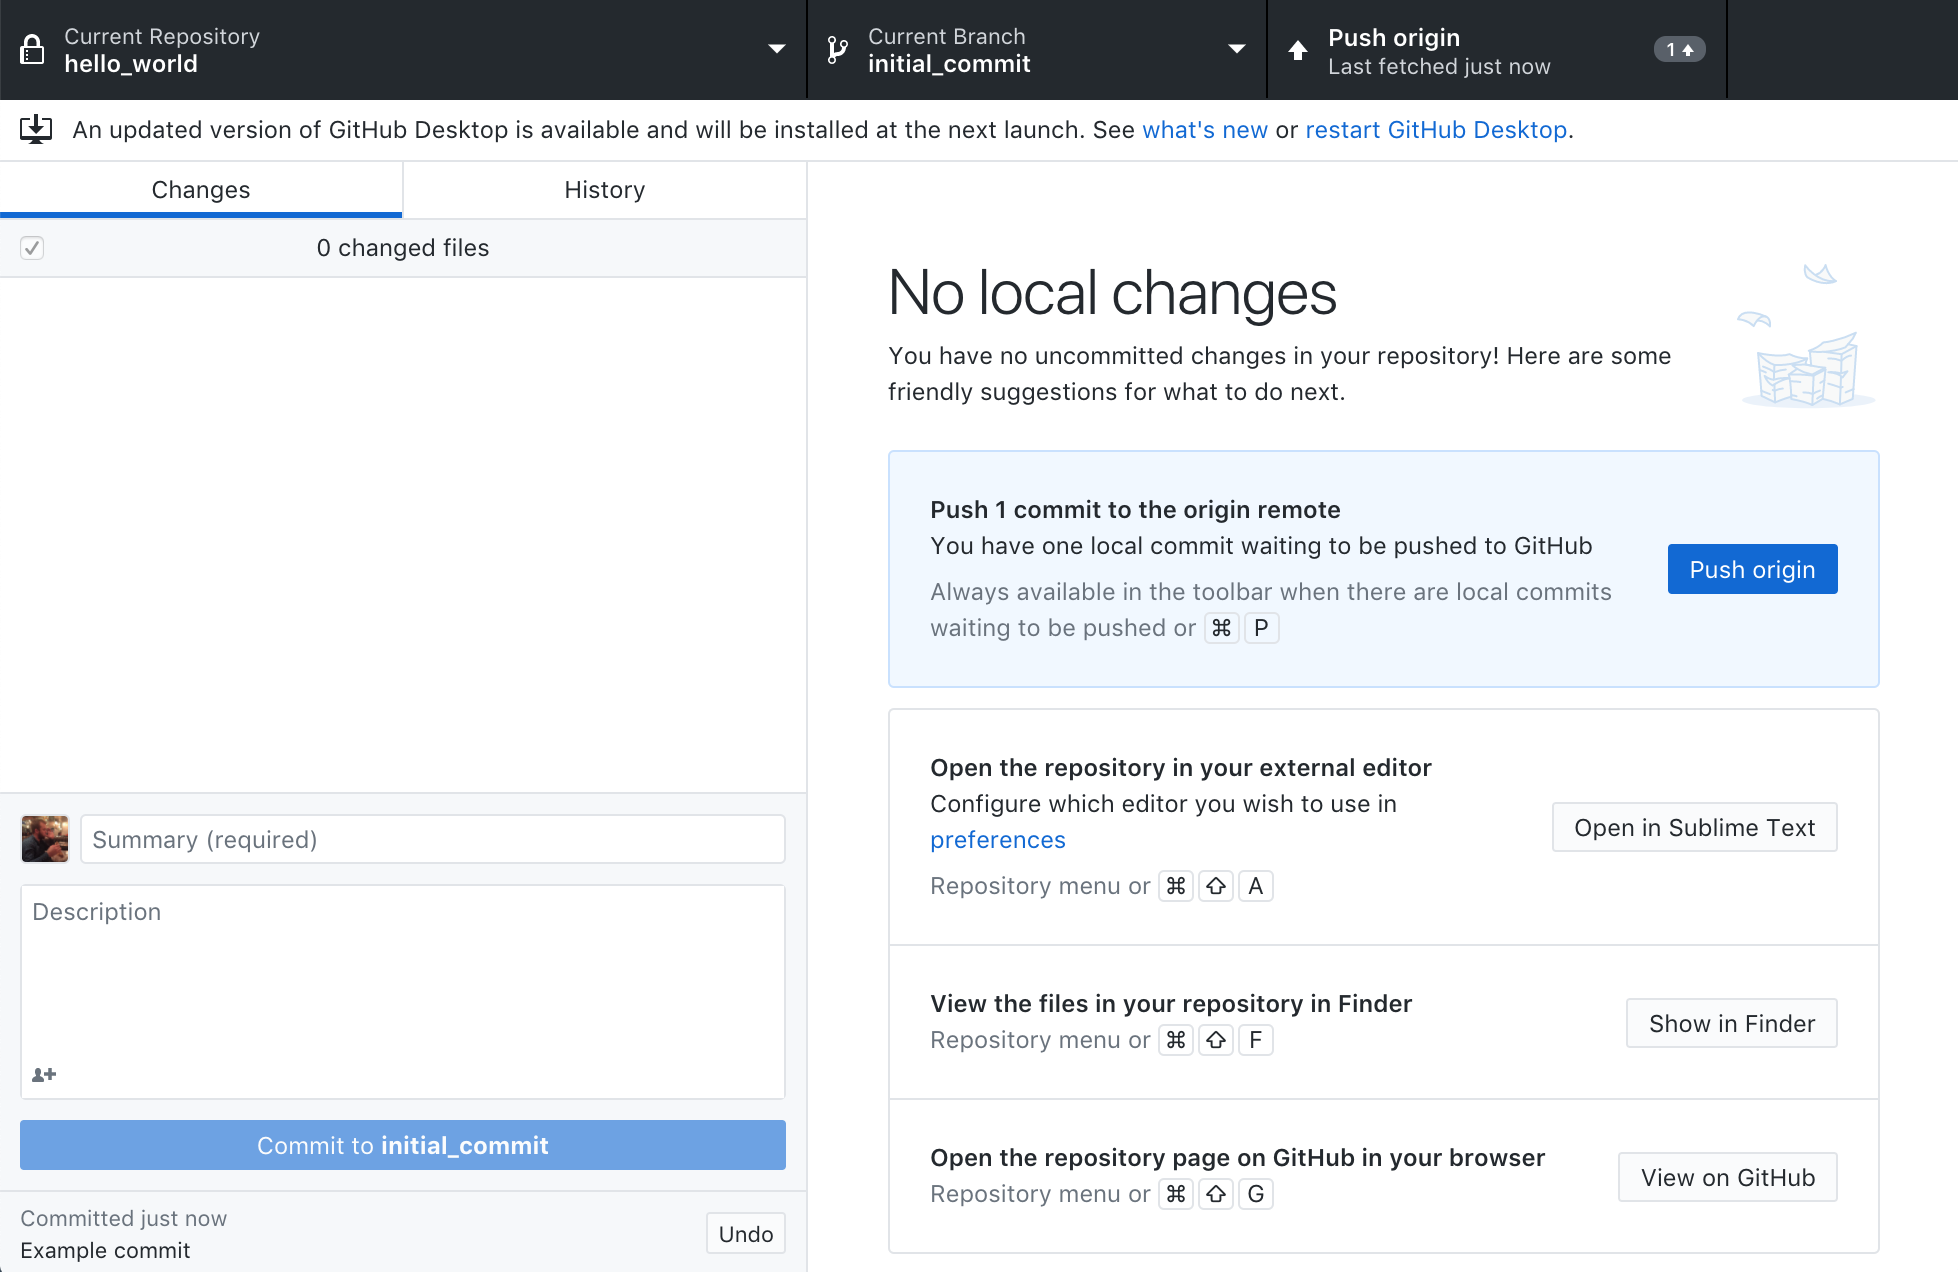
\includegraphics[width=.4\linewidth]{push_origin.png}
\end{subfigure}
\end{figure}
\end{frame}

\begin{frame}{Step 5: Open a pull request}
\begin{itemize}
    \item After pushing to origin, you are prompted to make a pull request for your work
    \item Making a pull request is making a request to merge your branch of code back into the master branch, or main codebase
    \item Before merging your pull request, all team members should review the changes and understand how new changes will affect the dependency structure
    \item Comment what changes you made on the pull request (important if you need to go back and review)
\end{itemize}
\begin{figure}
\centering
\begin{subfigure}{\textwidth}
  \centering
  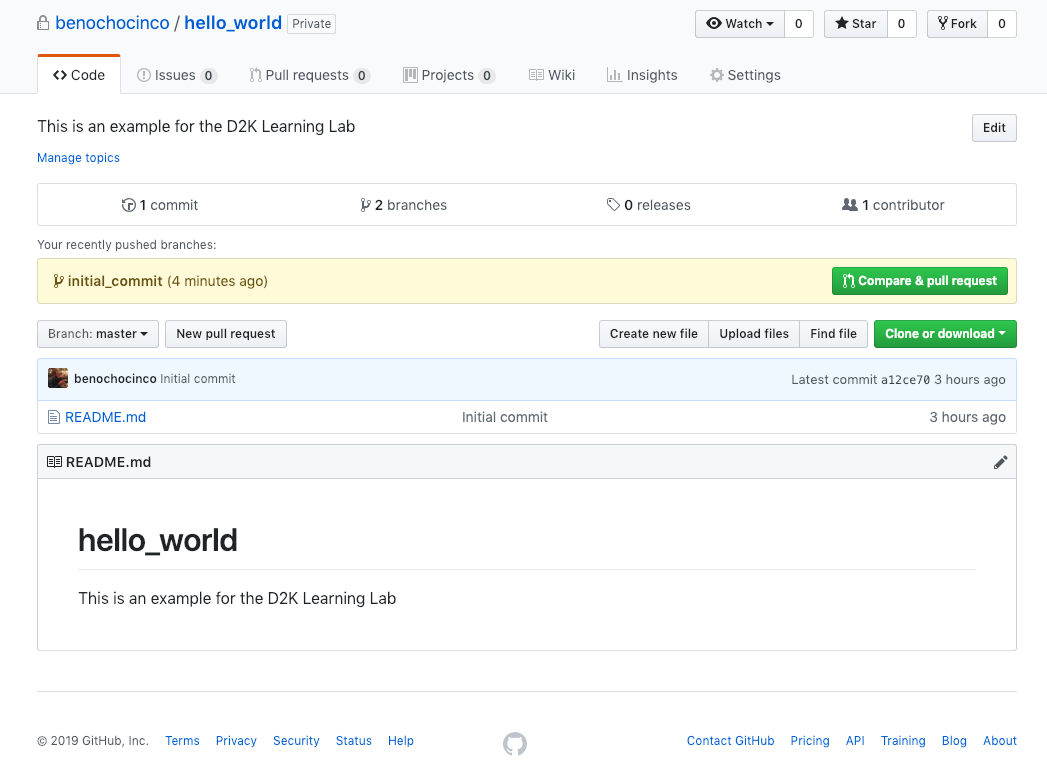
\includegraphics[width=.3\linewidth]{make_pr.png}
\end{subfigure}%
\begin{subfigure}{\textwidth}
  \centering
  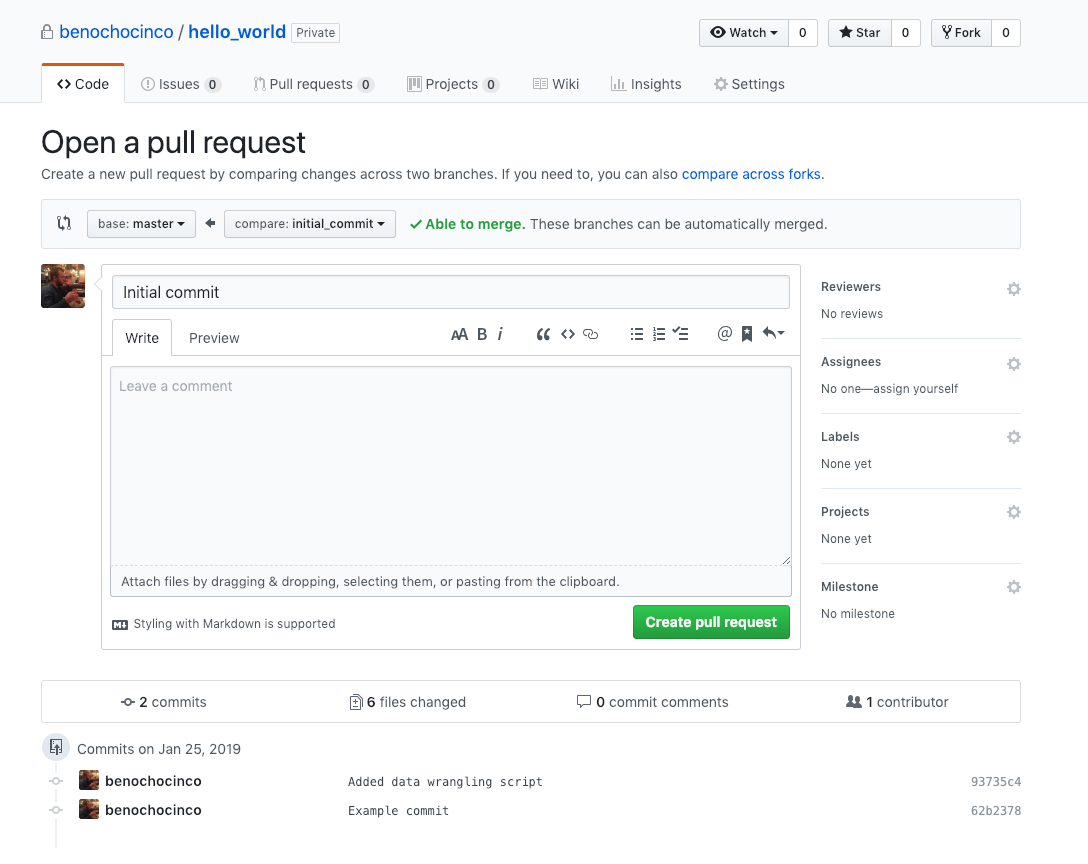
\includegraphics[width=.3\linewidth]{open_pr.png}
\end{subfigure}
\begin{subfigure}{\textwidth}
  \centering
  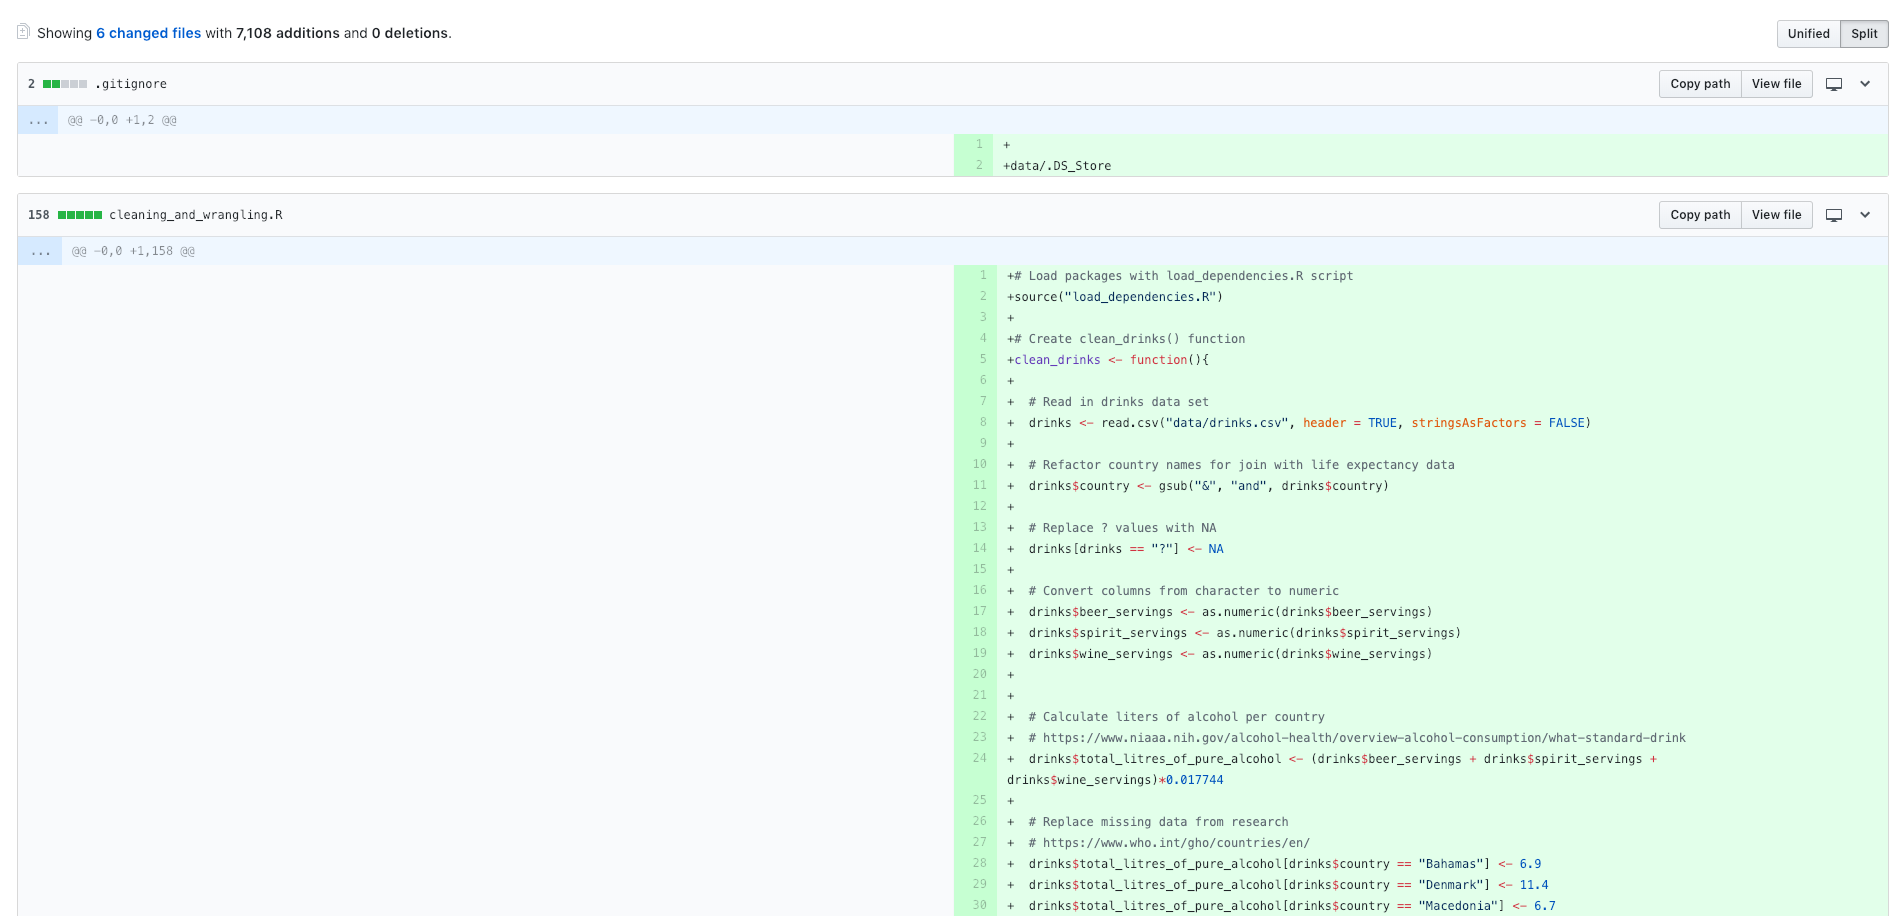
\includegraphics[width=.3\linewidth]{review_changes.png}
\end{subfigure}
\end{figure}
\end{frame}

\begin{frame}{Step 6: Merge your pull request}
\begin{itemize}
    \item Once you have opened a pull request you can merge it back into the master branch if there are no conflicts
    \item Merge conflicts occur when competing changes are made to the same line of a file (this could include deletion of the line)
    \item Merge conflicts are easy to avoid if you communicate with your teammates and always create new branches from the master branch when starting a new modularized task
\end{itemize}
\begin{figure}
\centering
\begin{subfigure}{\textwidth}
  \centering
  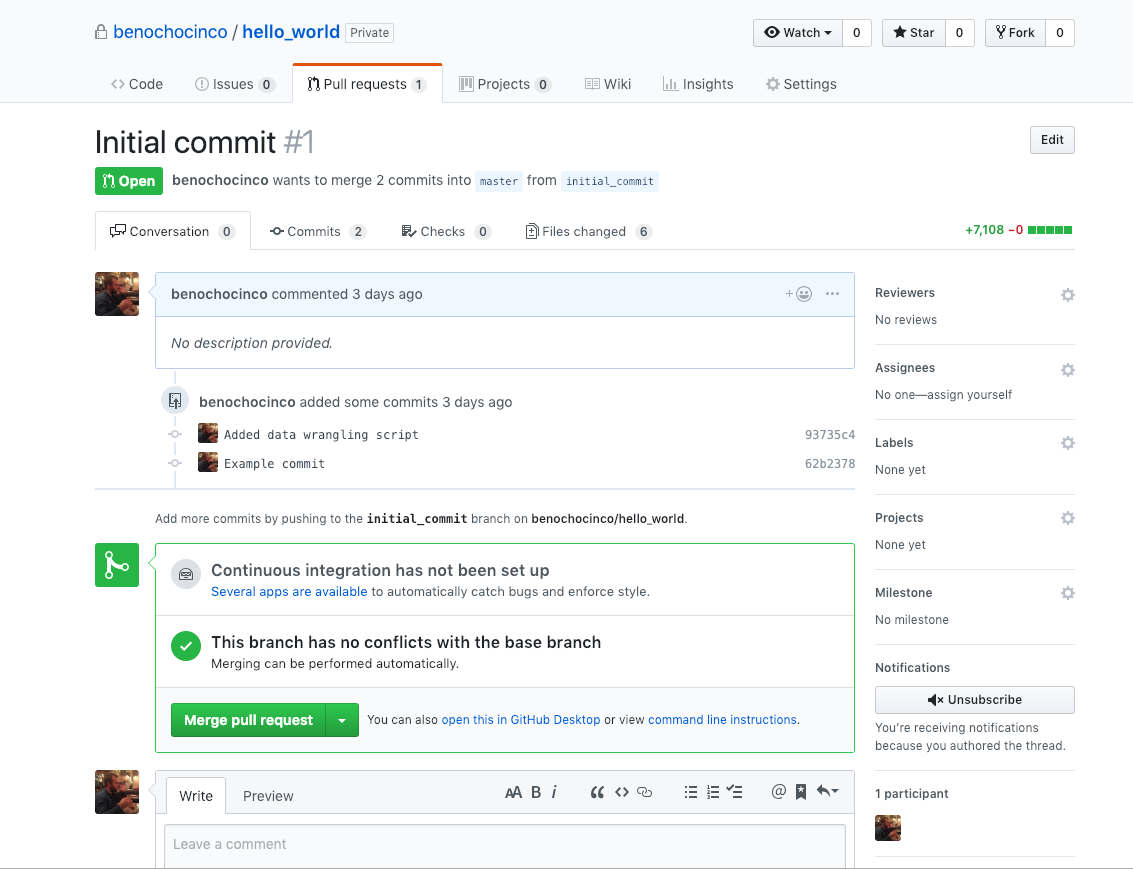
\includegraphics[width=.3\linewidth]{merge_branch.png}
\end{subfigure}%
\begin{subfigure}{\textwidth}
  \centering
  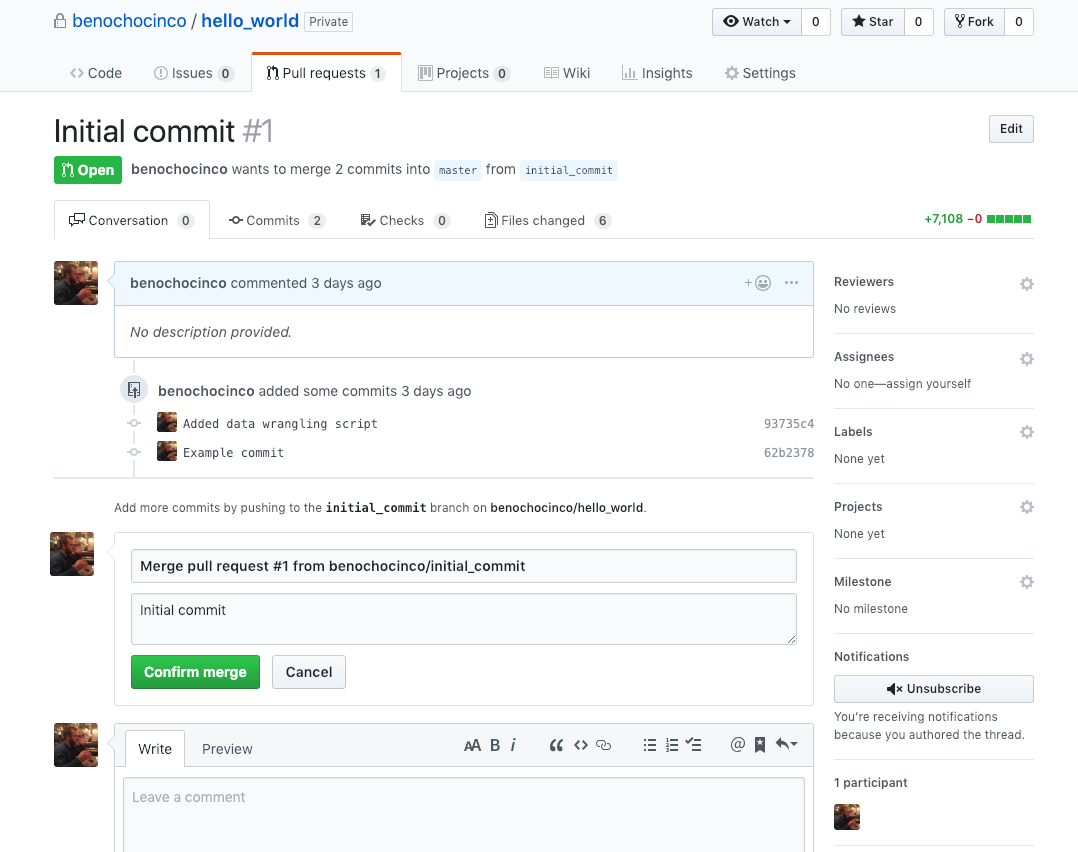
\includegraphics[width=.3\linewidth]{confirm_merge.png}
\end{subfigure}
\begin{subfigure}{\textwidth}
  \centering
  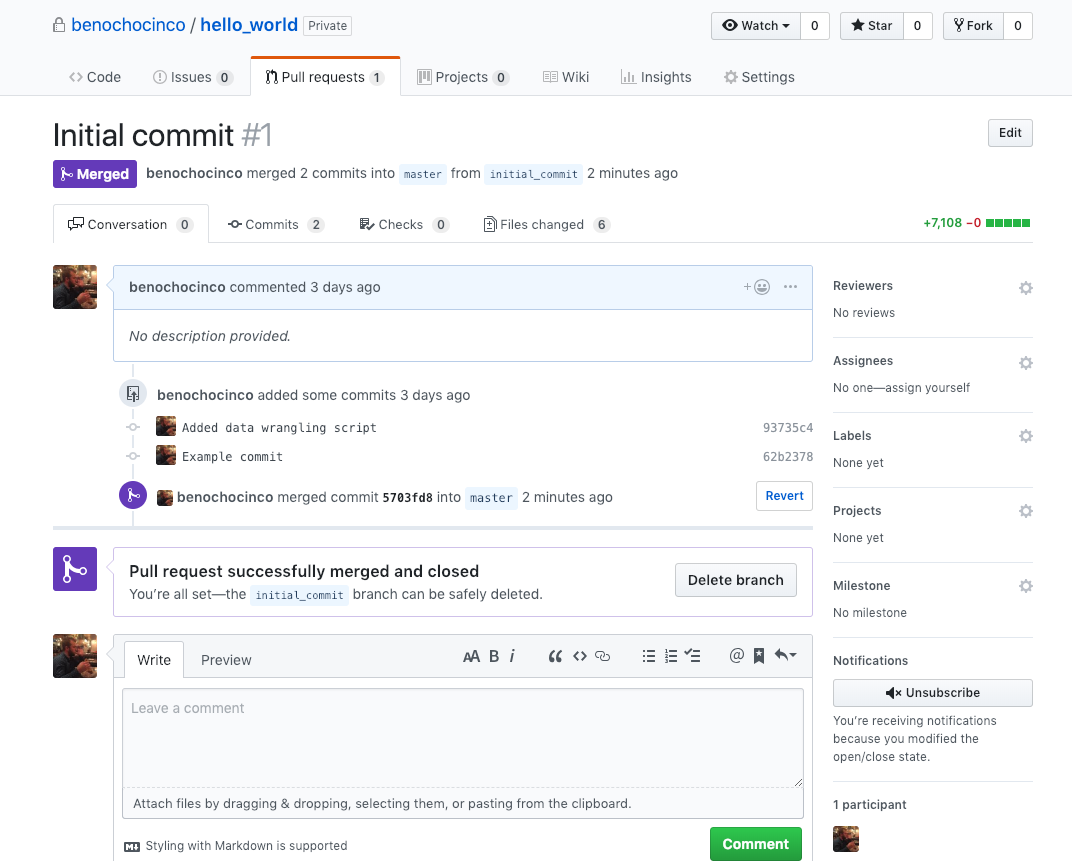
\includegraphics[width=.3\linewidth]{confirmed_merge.png}
\end{subfigure}
\end{figure}
\end{frame}

\begin{frame}{Resolving Merge Conflicts}
\begin{itemize}
    \item Merge conflicts \textbf{will} happen at some point this semester, \textbf{DON'T FREAK OUT!}
    \item Most likely caused by someone committing, pushing, pulling and merging a change to the same files or lines you have changed on your branch
    \item Example:
    \begin{itemize}
        \item Added a line of code on the \textbf{create\_merge\_conflict} branch then committed, pushed, pulled, merged with master branch
        \item Changed same line of code on outdated \textbf{conflict\_branch} branch then committed and pushed
    \end{itemize}
\end{itemize}
\begin{figure}
\centering
\begin{subfigure}{\textwidth}
  \centering
  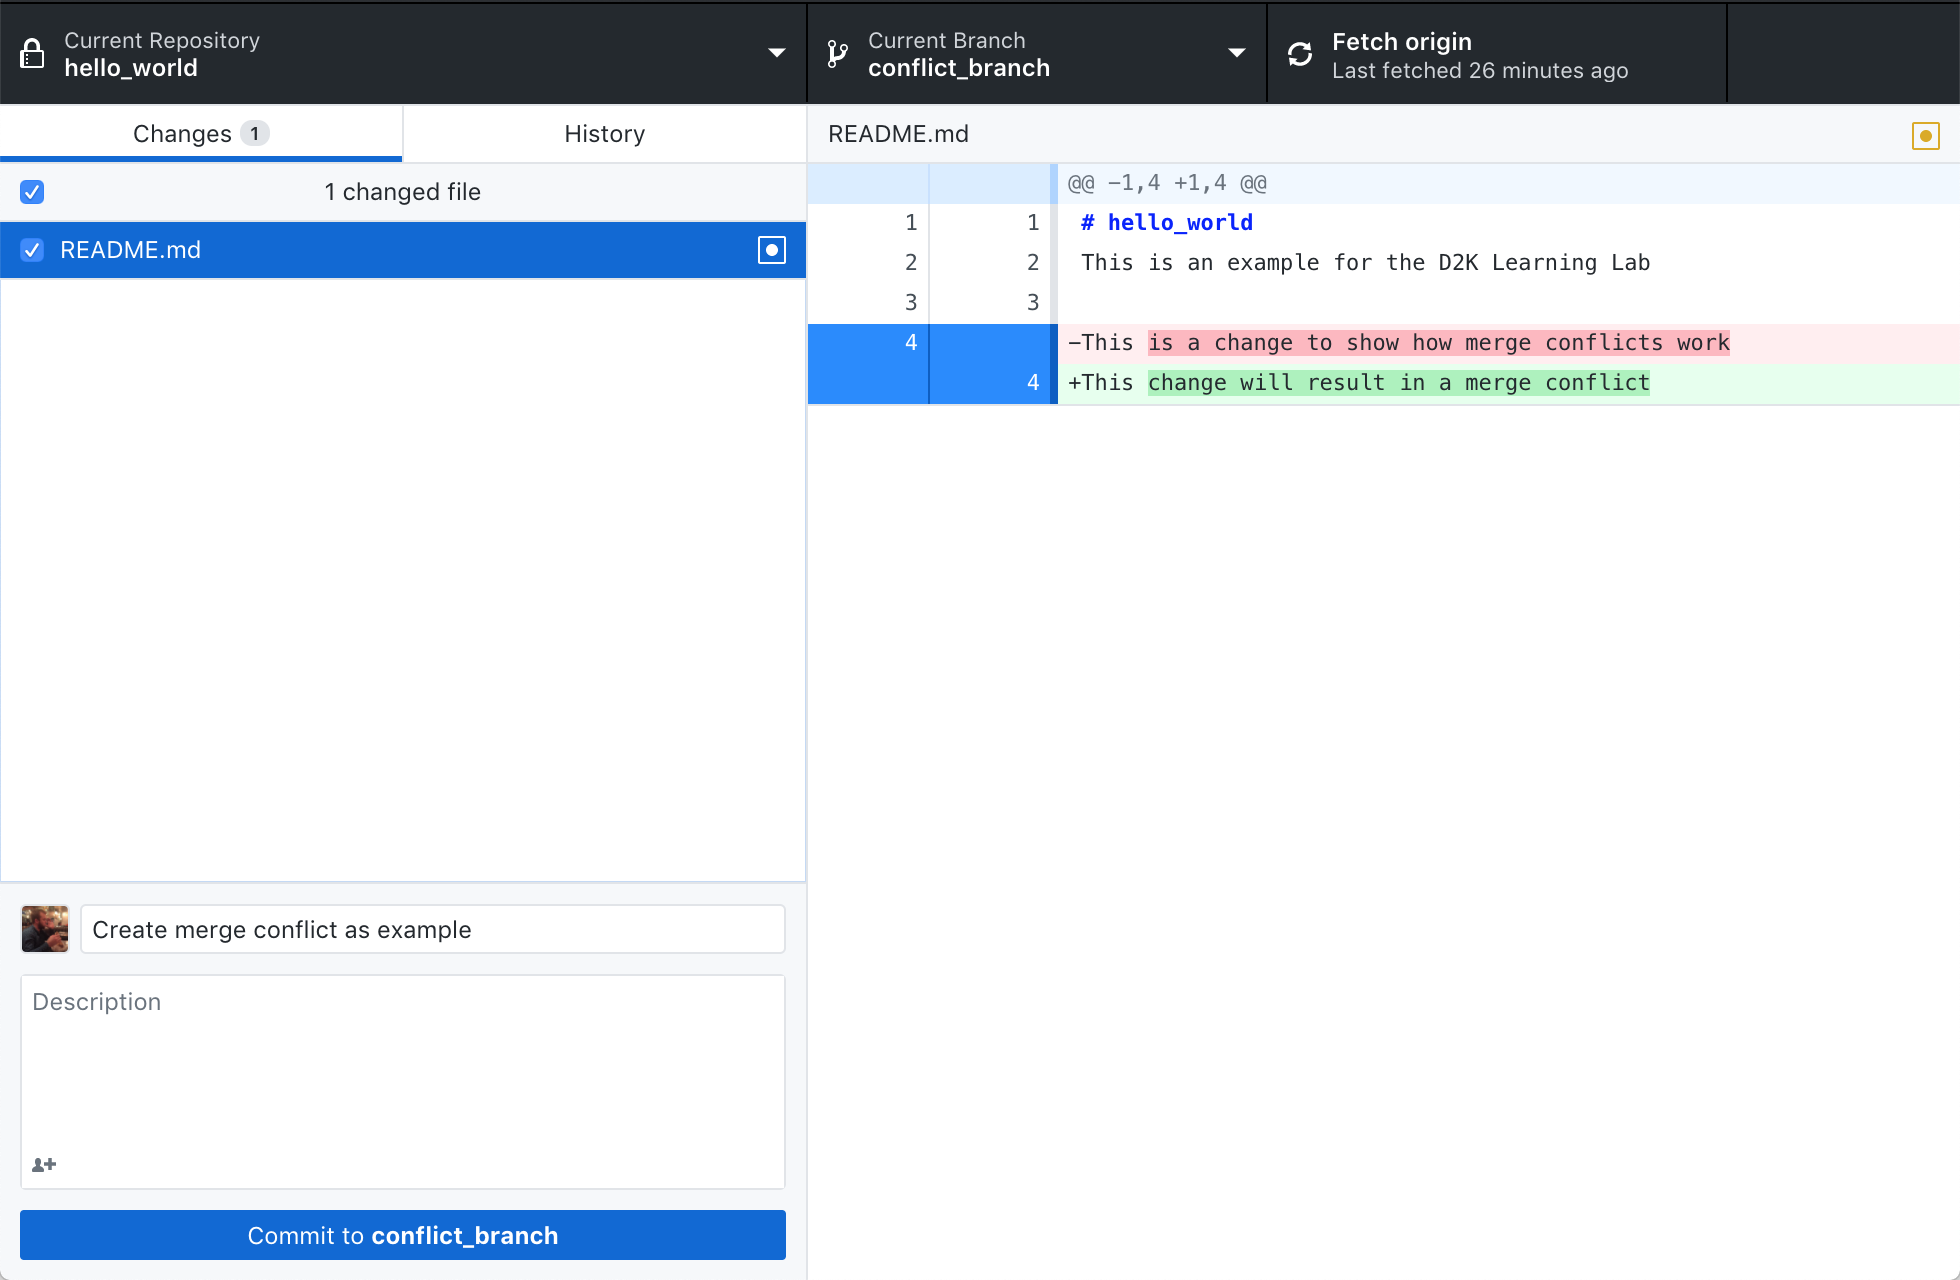
\includegraphics[width=.4\linewidth]{create_conflict.png}
\end{subfigure}%
\hspace{1cm}
\begin{subfigure}{\textwidth}
  \centering
  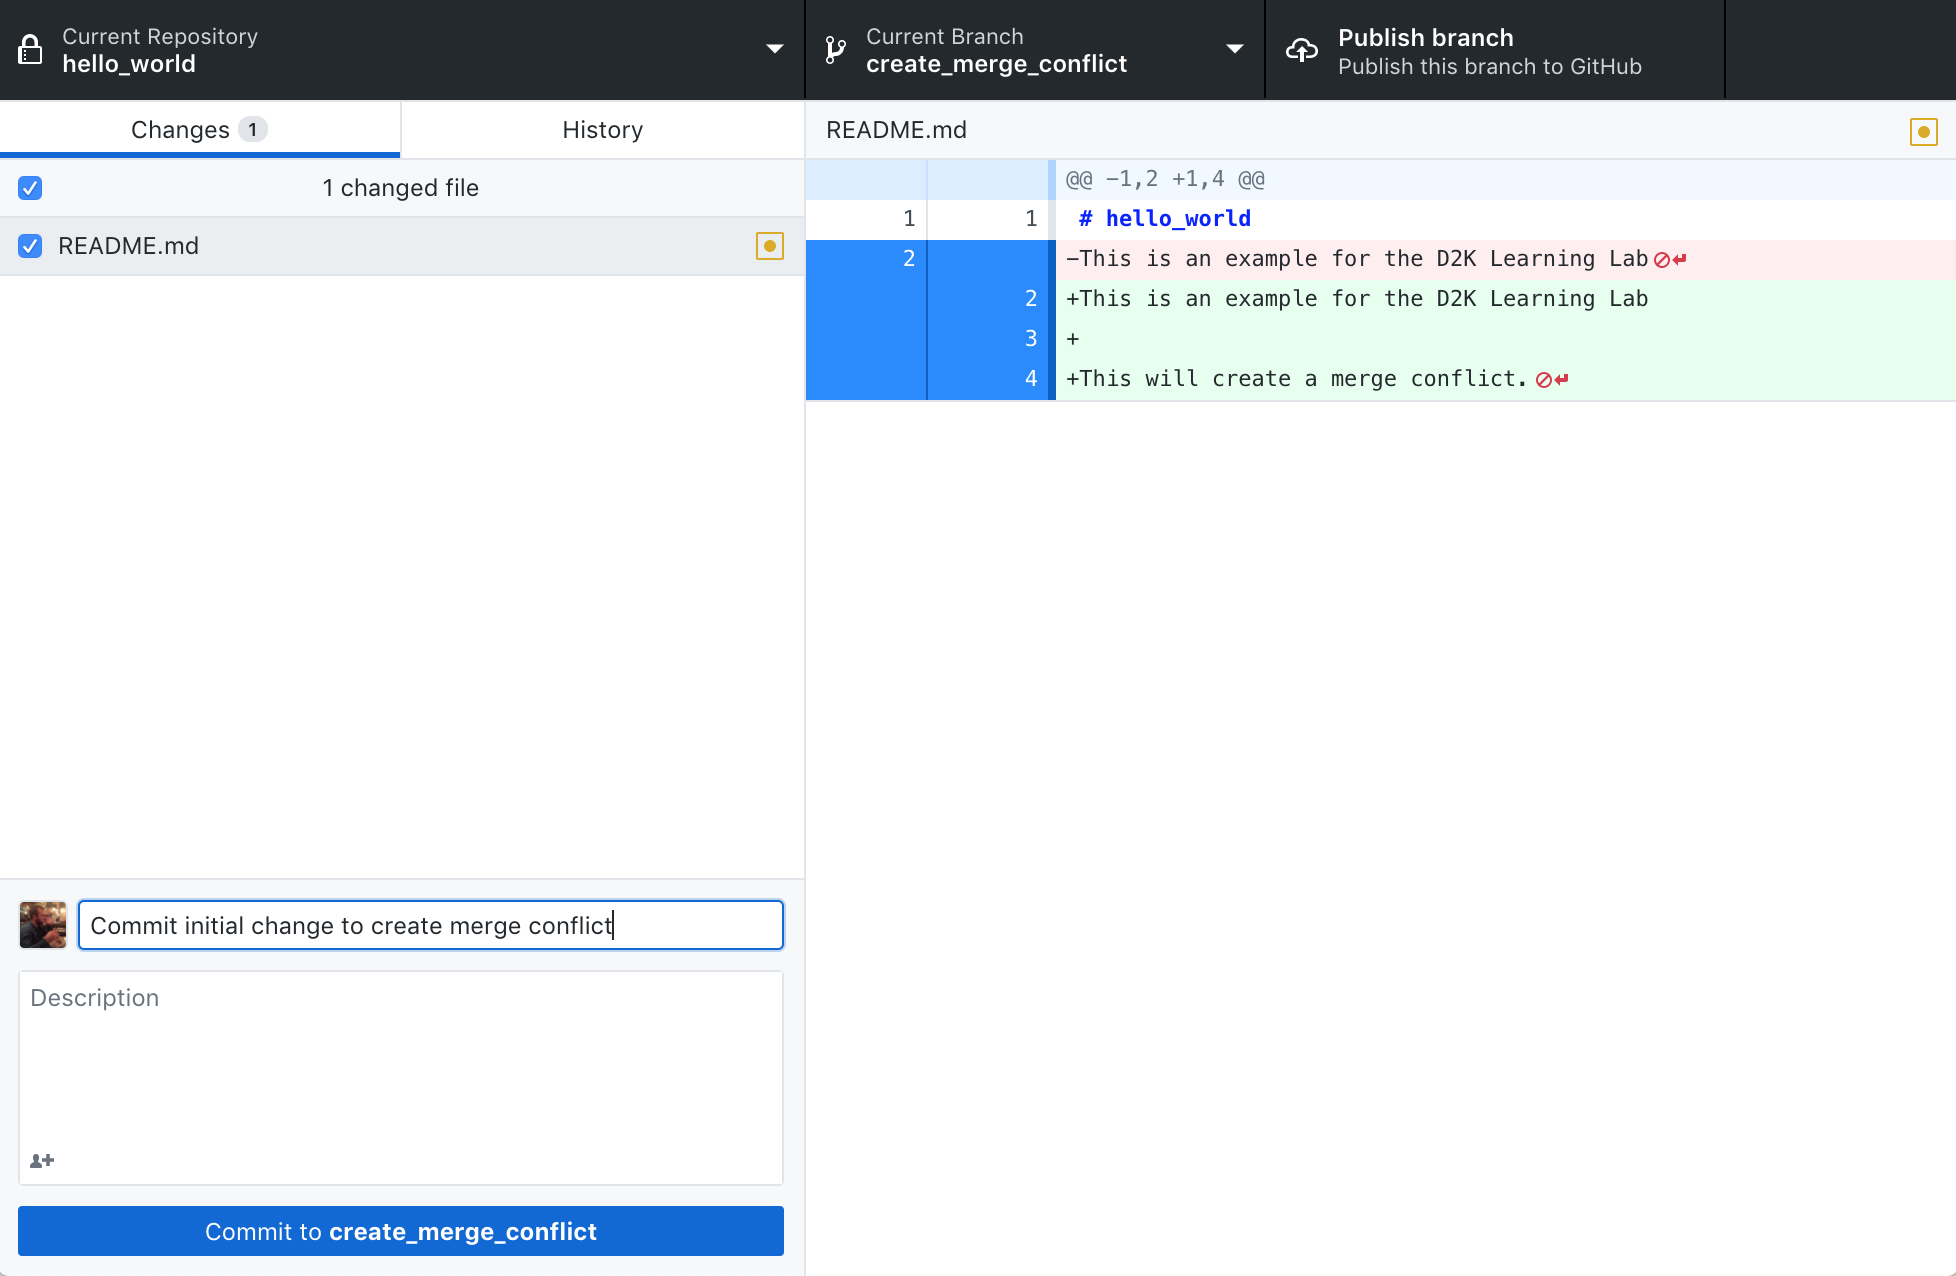
\includegraphics[width=.4\linewidth]{create_merge_conflict.png}
\end{subfigure}
\end{figure}
\end{frame}

\begin{frame}{Resolving Merge Conflicts}
\begin{itemize}
    \item After pushing the new branch that creates the conflict, you can still open a pull request to review the code
    \item Once the new pull request has been opened, click on \textbf{Resolve conflicts} to review the conflict and reconcile the differences
\end{itemize}
\begin{figure}
\centering
\begin{subfigure}{\textwidth}
  \centering
  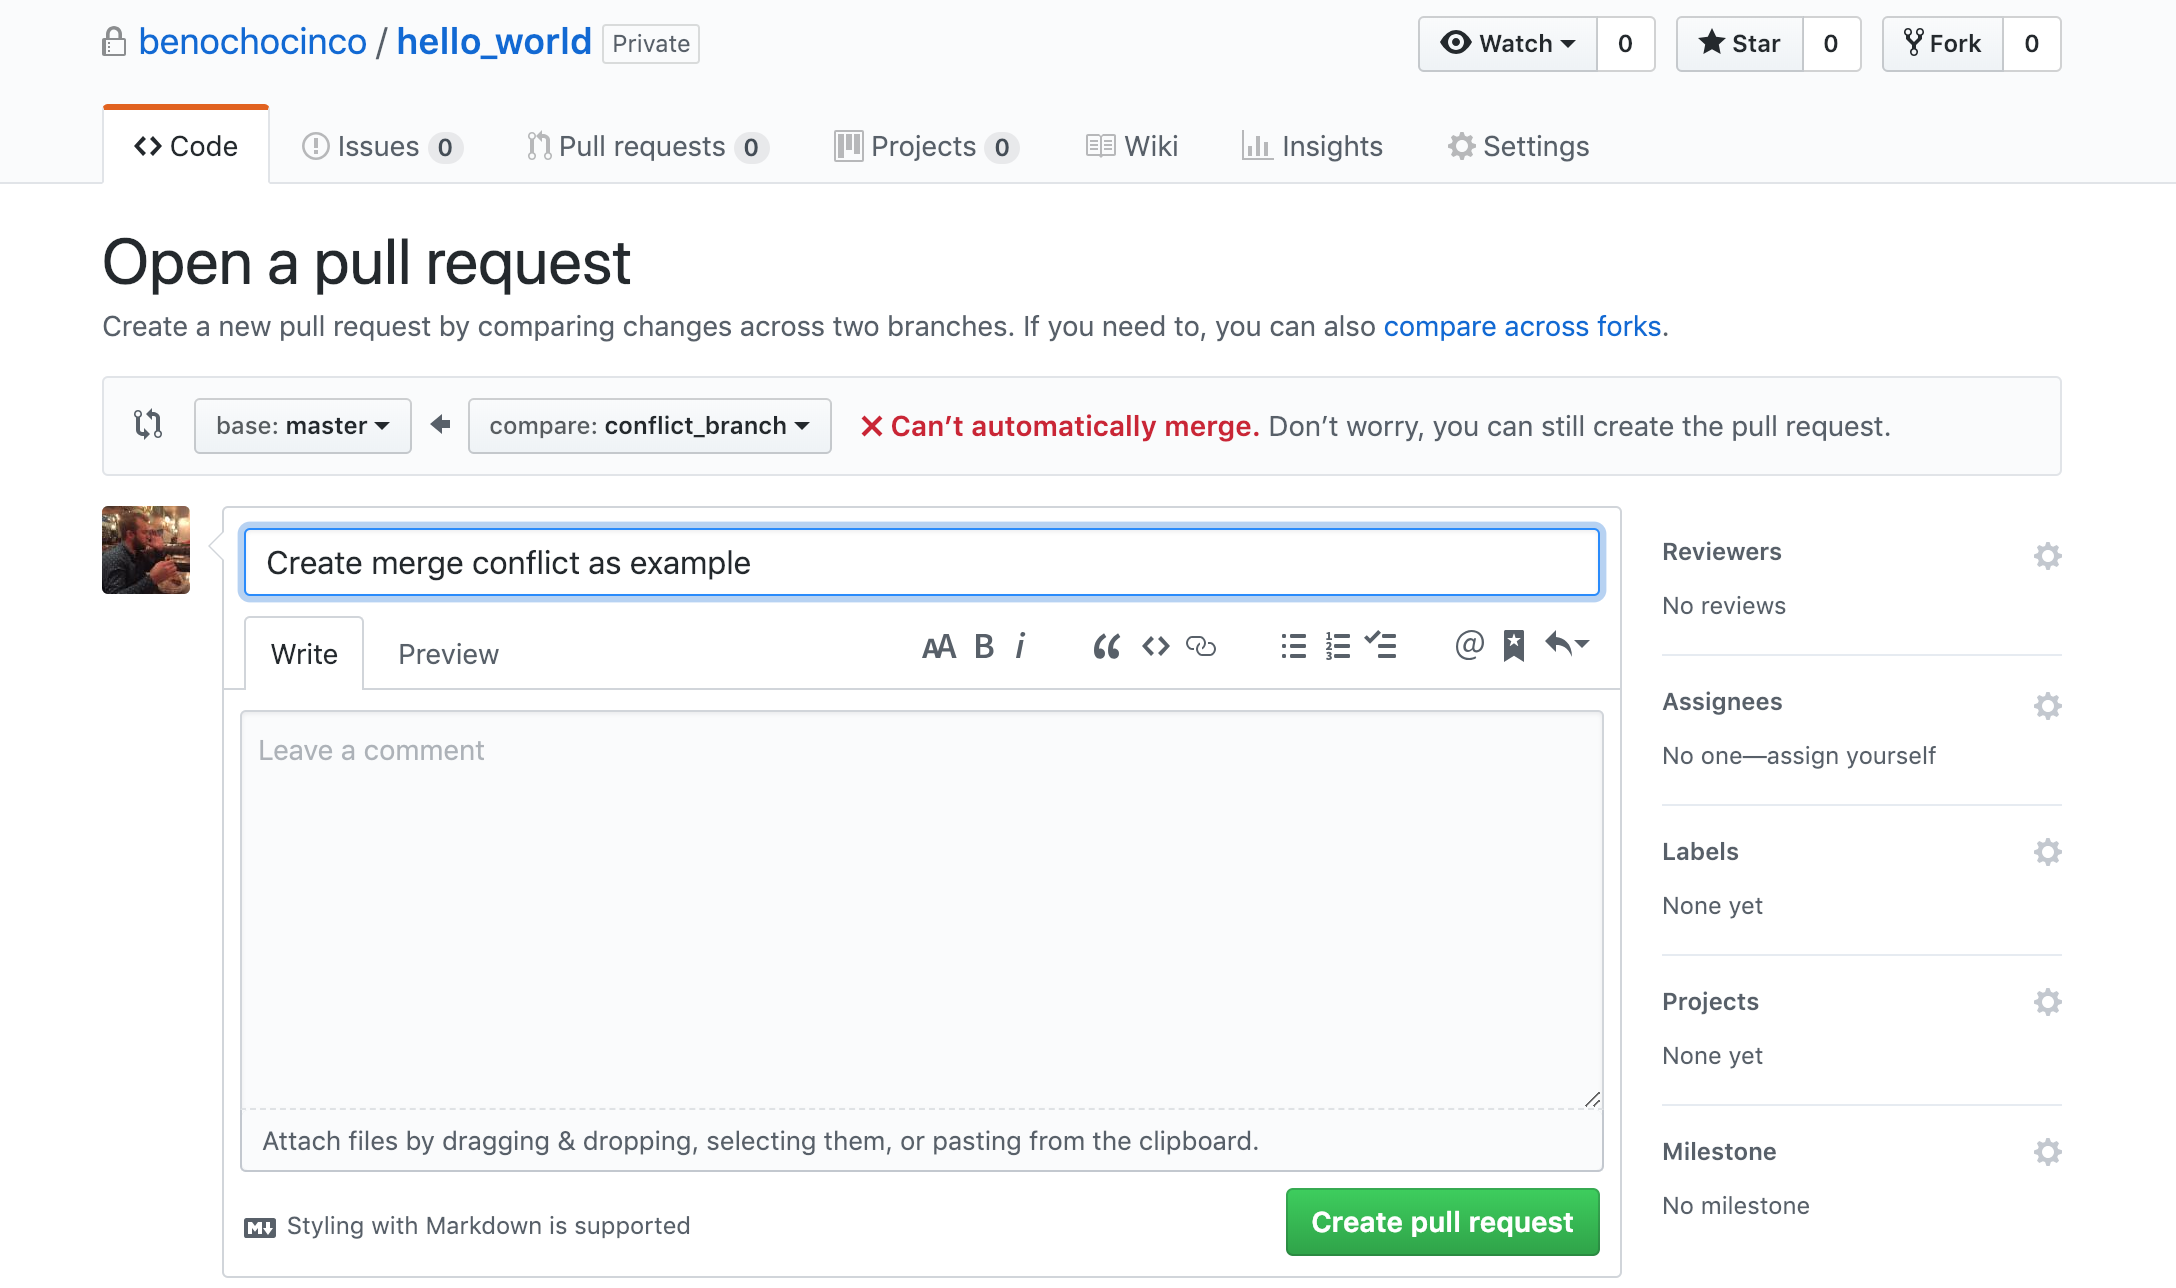
\includegraphics[width=.4\linewidth]{open_conflict_pr.png}
\end{subfigure}%
\hspace{1cm}
\begin{subfigure}{\textwidth}
  \centering
  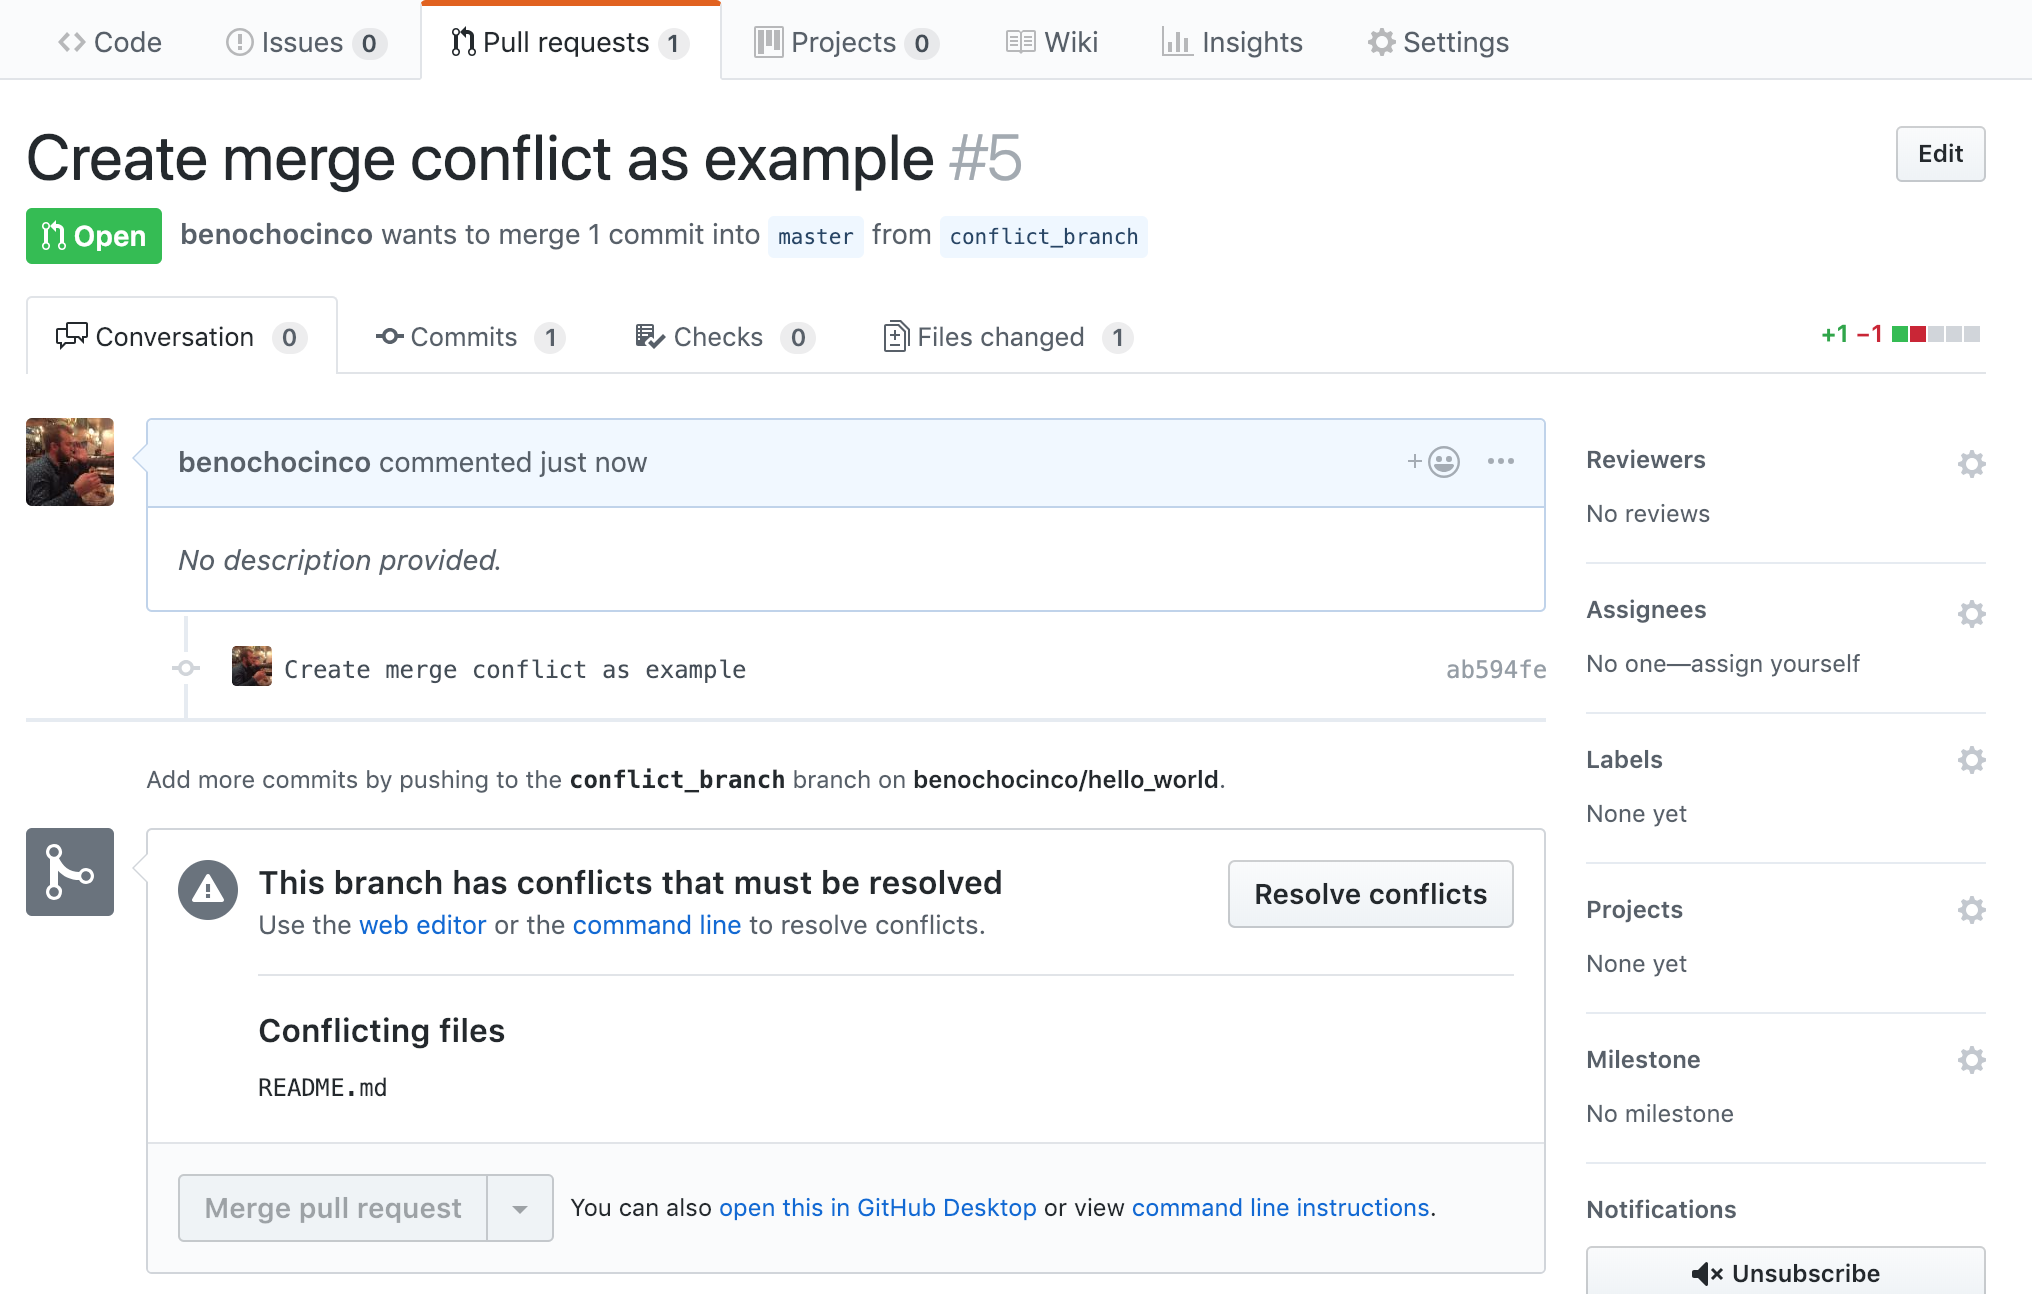
\includegraphics[width=.4\linewidth]{resolve_conflicts.png}
\end{subfigure}
\end{figure}
\end{frame}

\begin{frame}{Resolving Merge Conflicts}
\begin{itemize}
    \item The changes on the base branch (HEAD branch) will be reflected on the line after $<<<<<<< HEAD$ and before $=======$
    \item The changes to the new feature branch which created the conflict will be represented after $=======$ and before $>>>>>>> BRANCH-NAME$
    \item To resolve the conflict, keep the change you want to be in your master branch and get rid of the $<<<<<<< HEAD$, $=======$, $>>>>>>> BRANCH-NAME$ conflict markers
\end{itemize}
\begin{figure}
\centering
\begin{subfigure}{\textwidth}
  \centering
  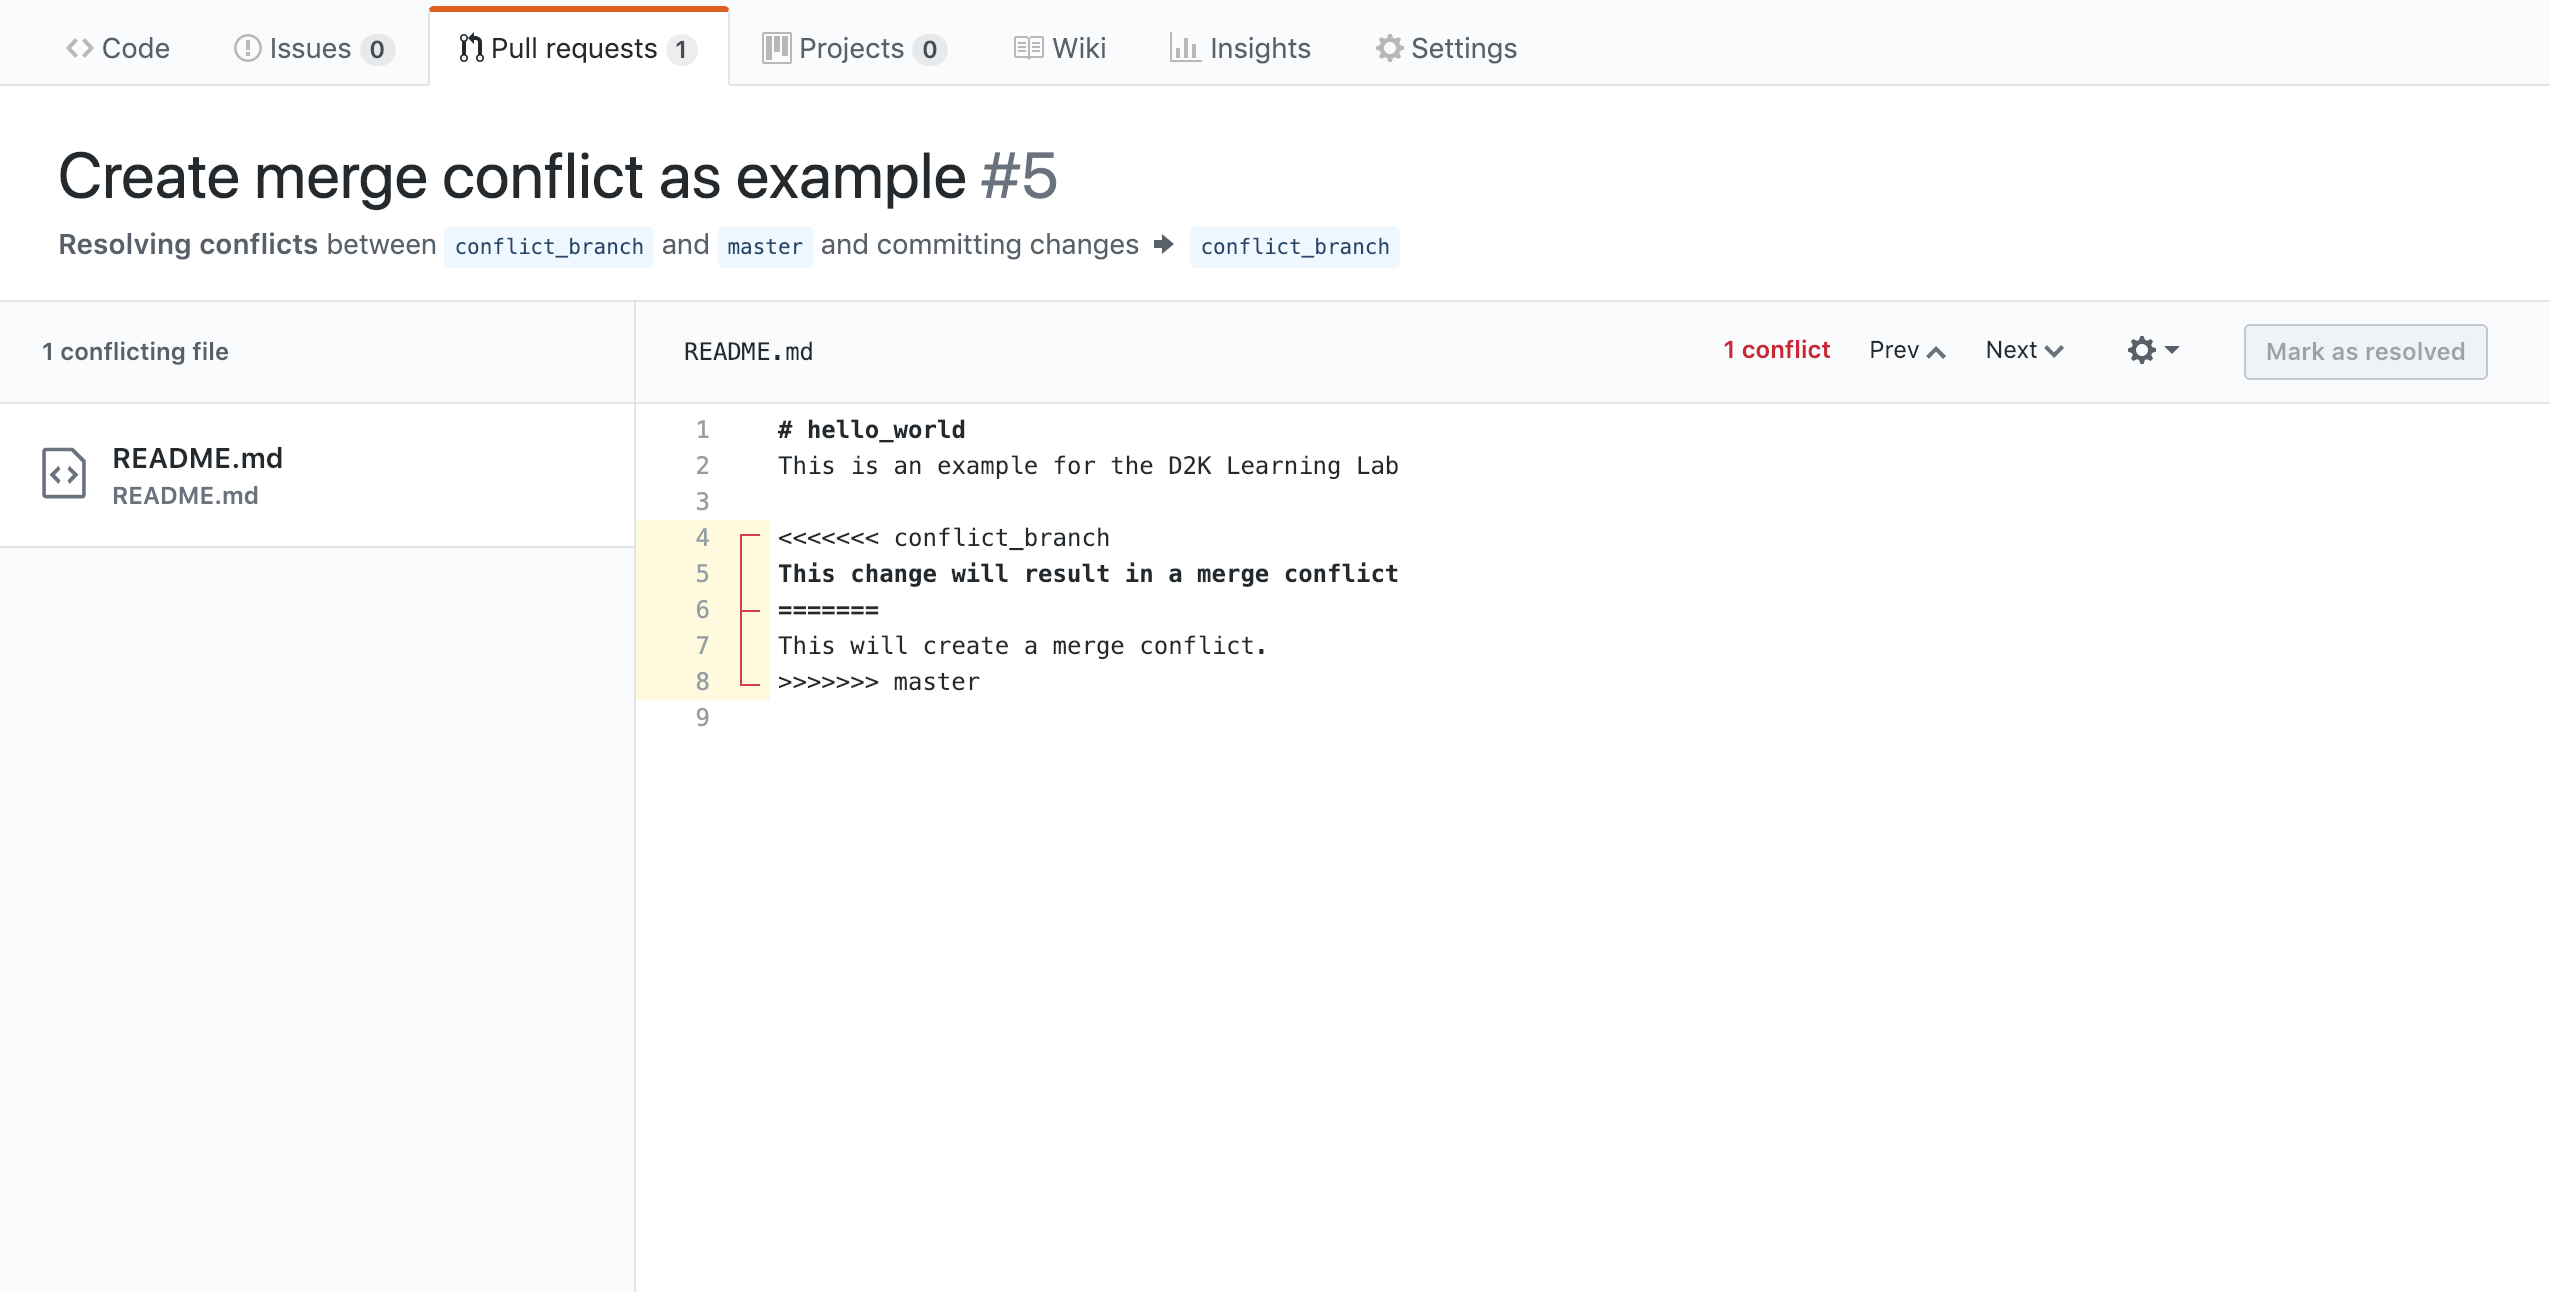
\includegraphics[width=.4\linewidth]{resolve1.png}
\end{subfigure}%
\hspace{1cm}
\begin{subfigure}{\textwidth}
  \centering
  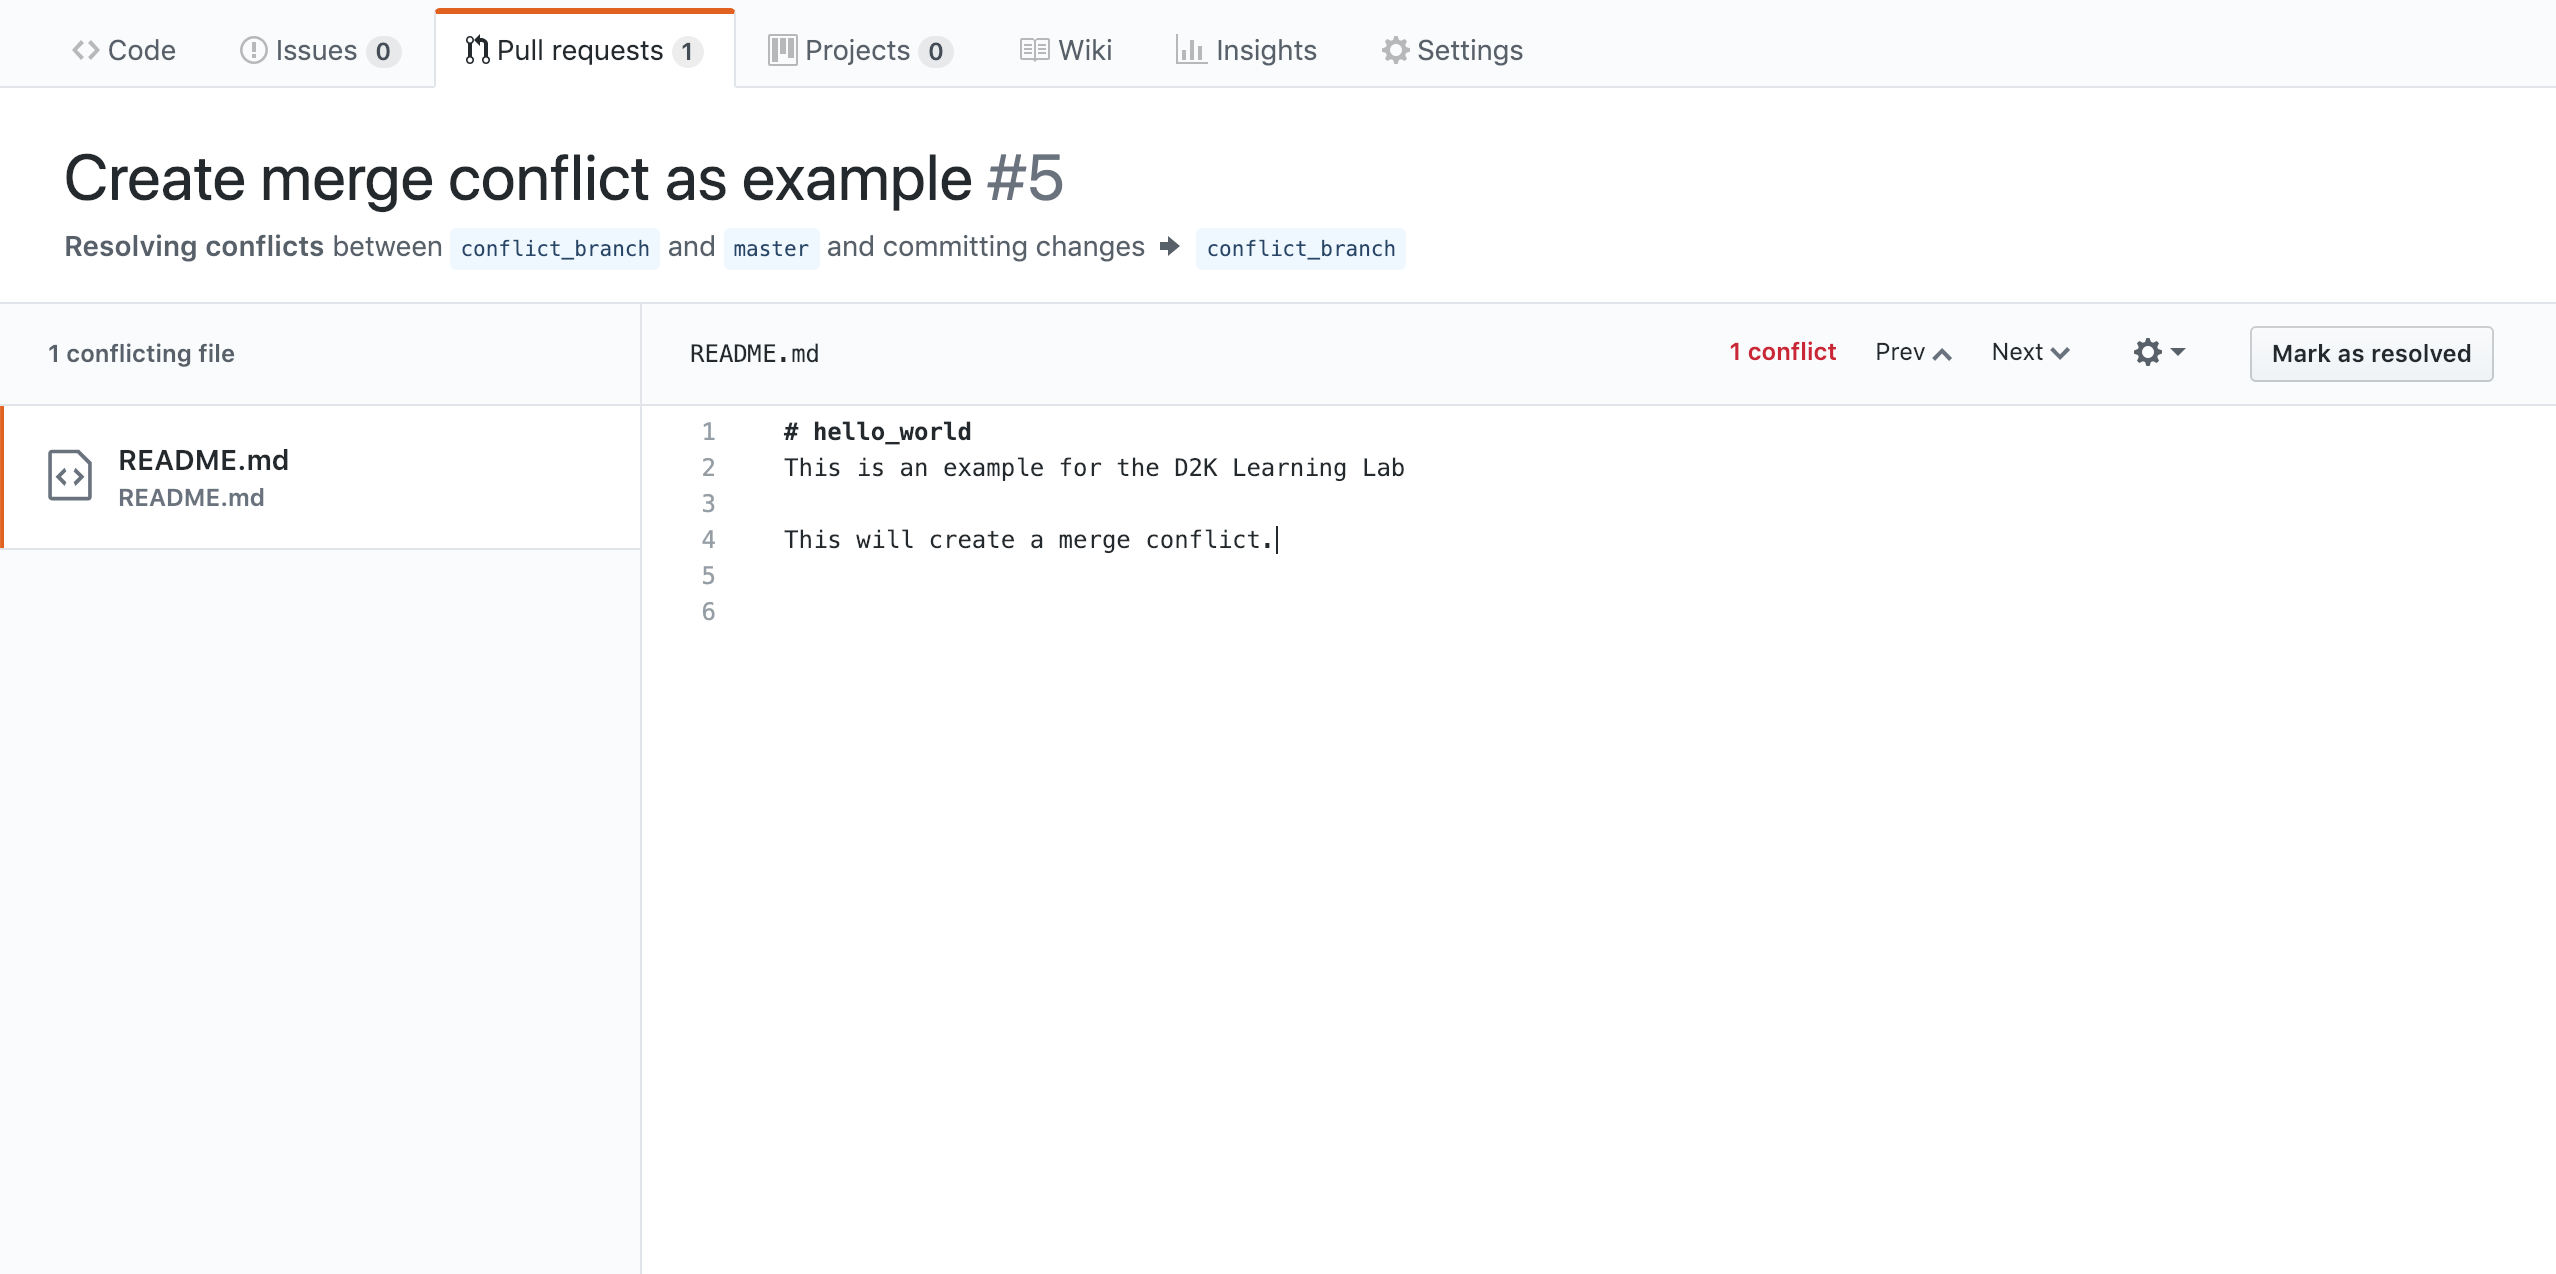
\includegraphics[width=.4\linewidth]{resolve2.png}
\end{subfigure}
\end{figure}
\end{frame}

\begin{frame}{Resolving Merge Conflicts}
\begin{itemize}
    \item After removing the conflict markers, you will be prompted to commit merge, do this
    \item Now you will be able to merge your original pull request without conflict
    \item Now that we have witnessed how much of a pain it is to resolve conflicts, we will do a better job in the future of not working from outdated branches!
\end{itemize}
\begin{figure}
\centering
\begin{subfigure}{\textwidth}
  \centering
  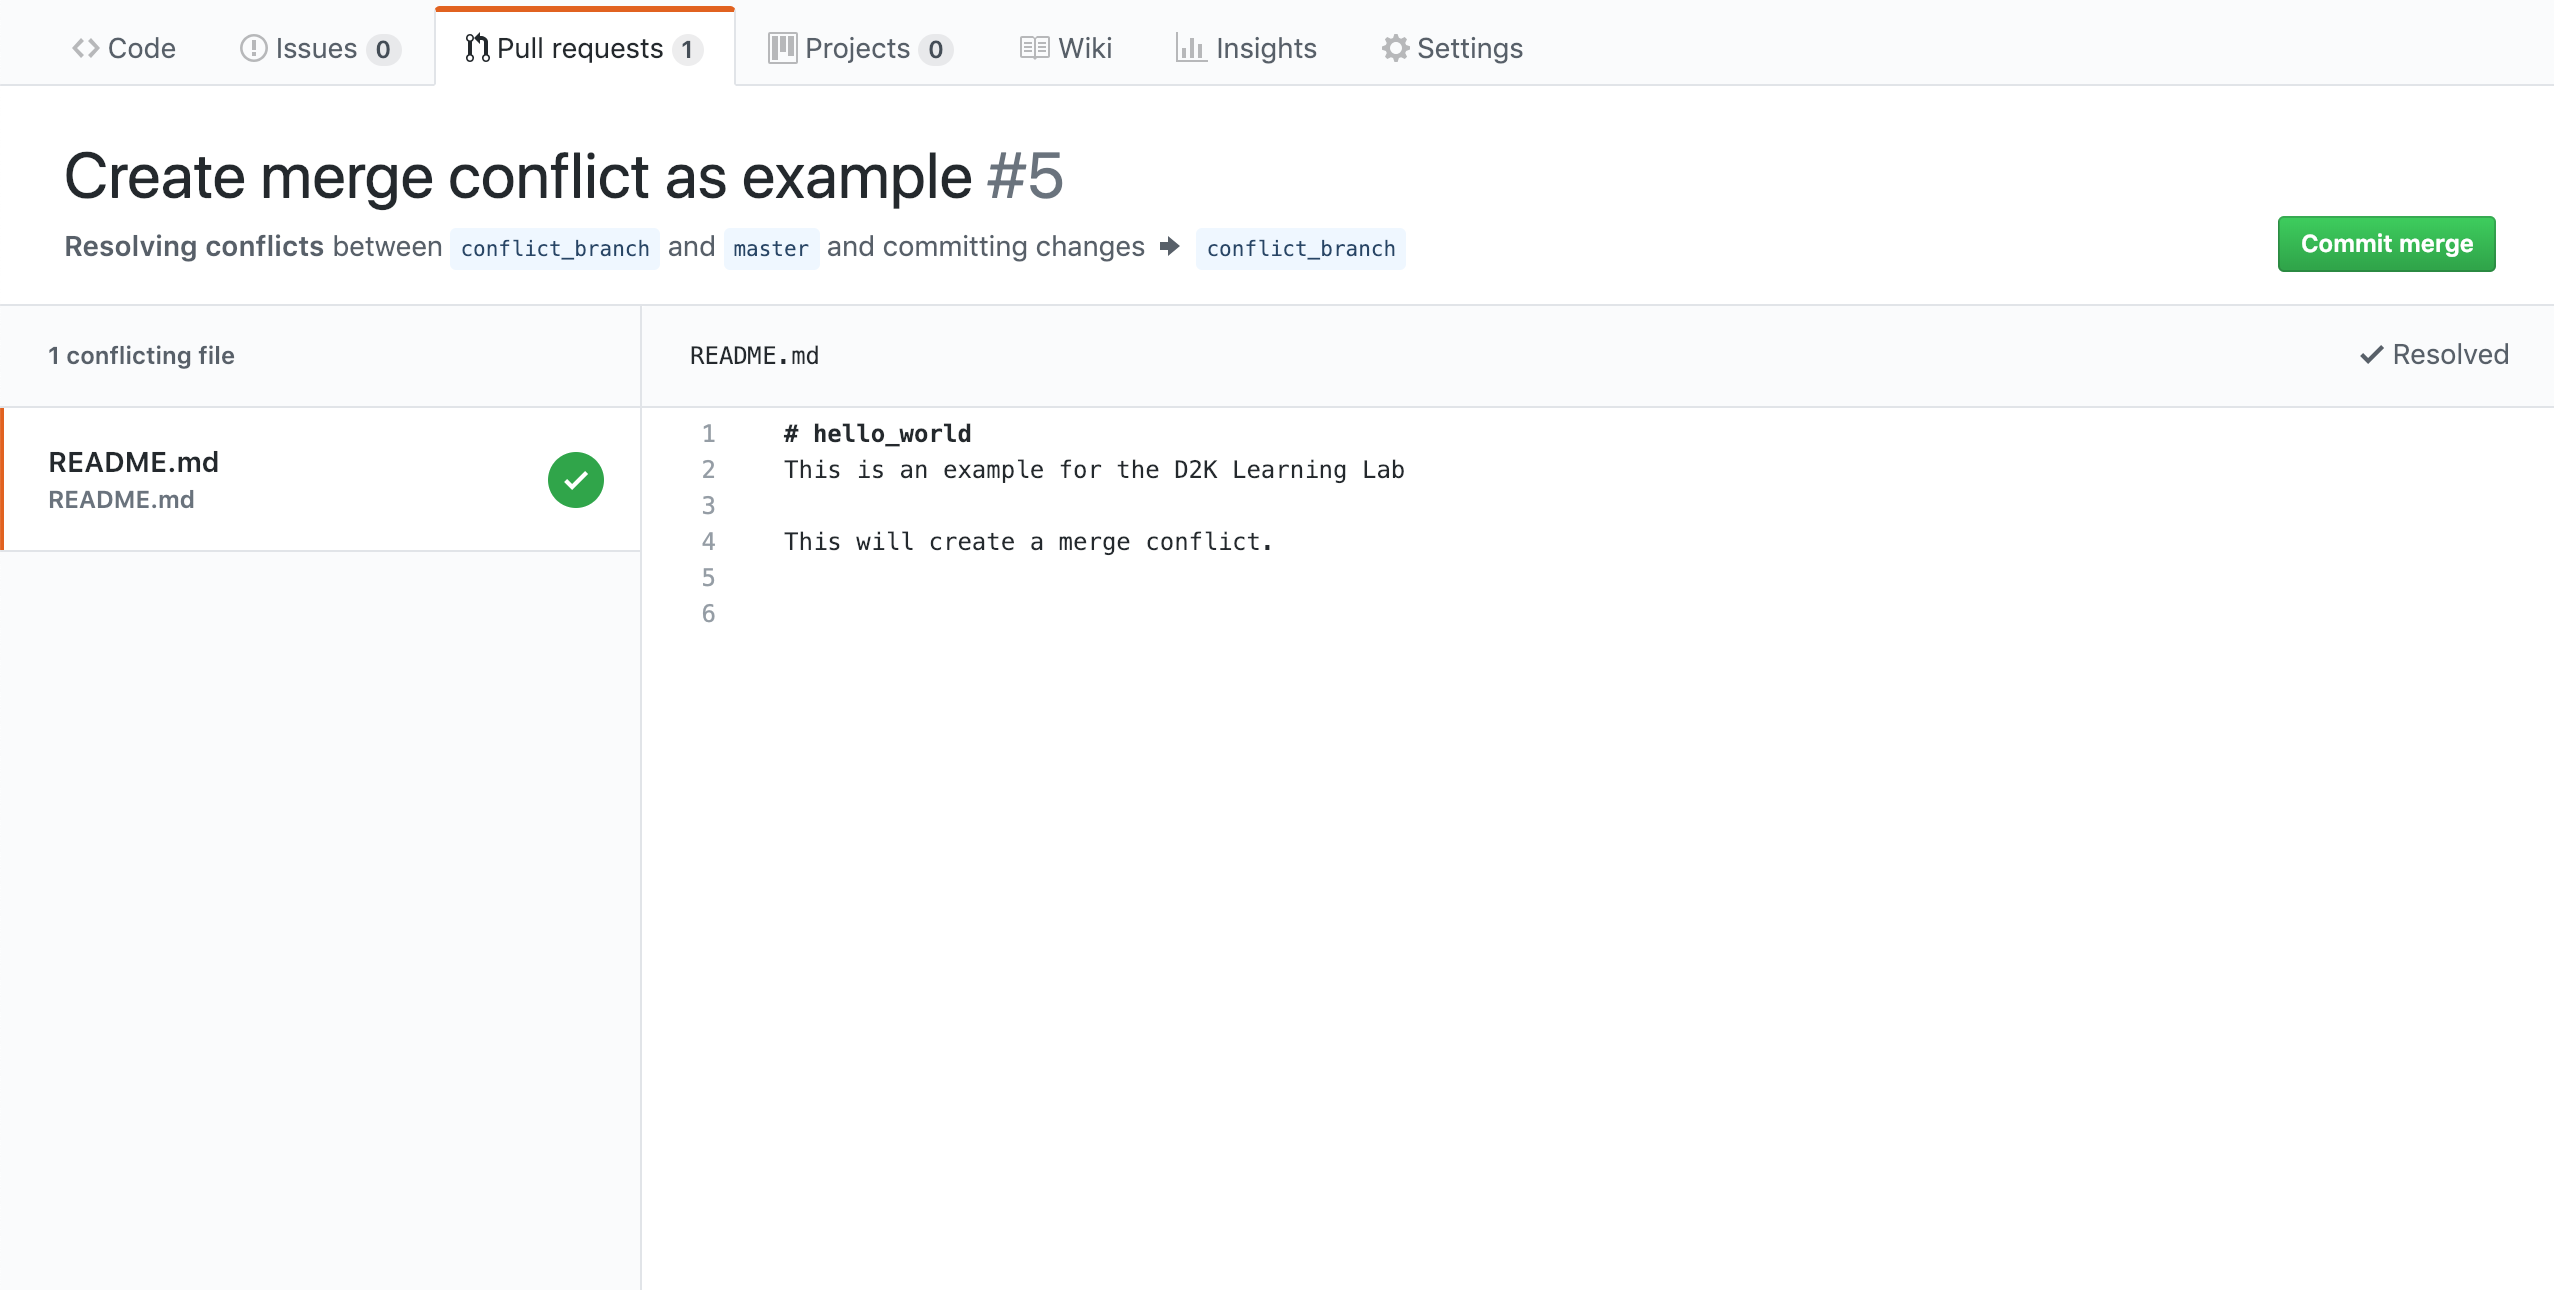
\includegraphics[width=.4\linewidth]{commit_merge.png}
\end{subfigure}%
\hspace{1cm}
\begin{subfigure}{\textwidth}
  \centering
  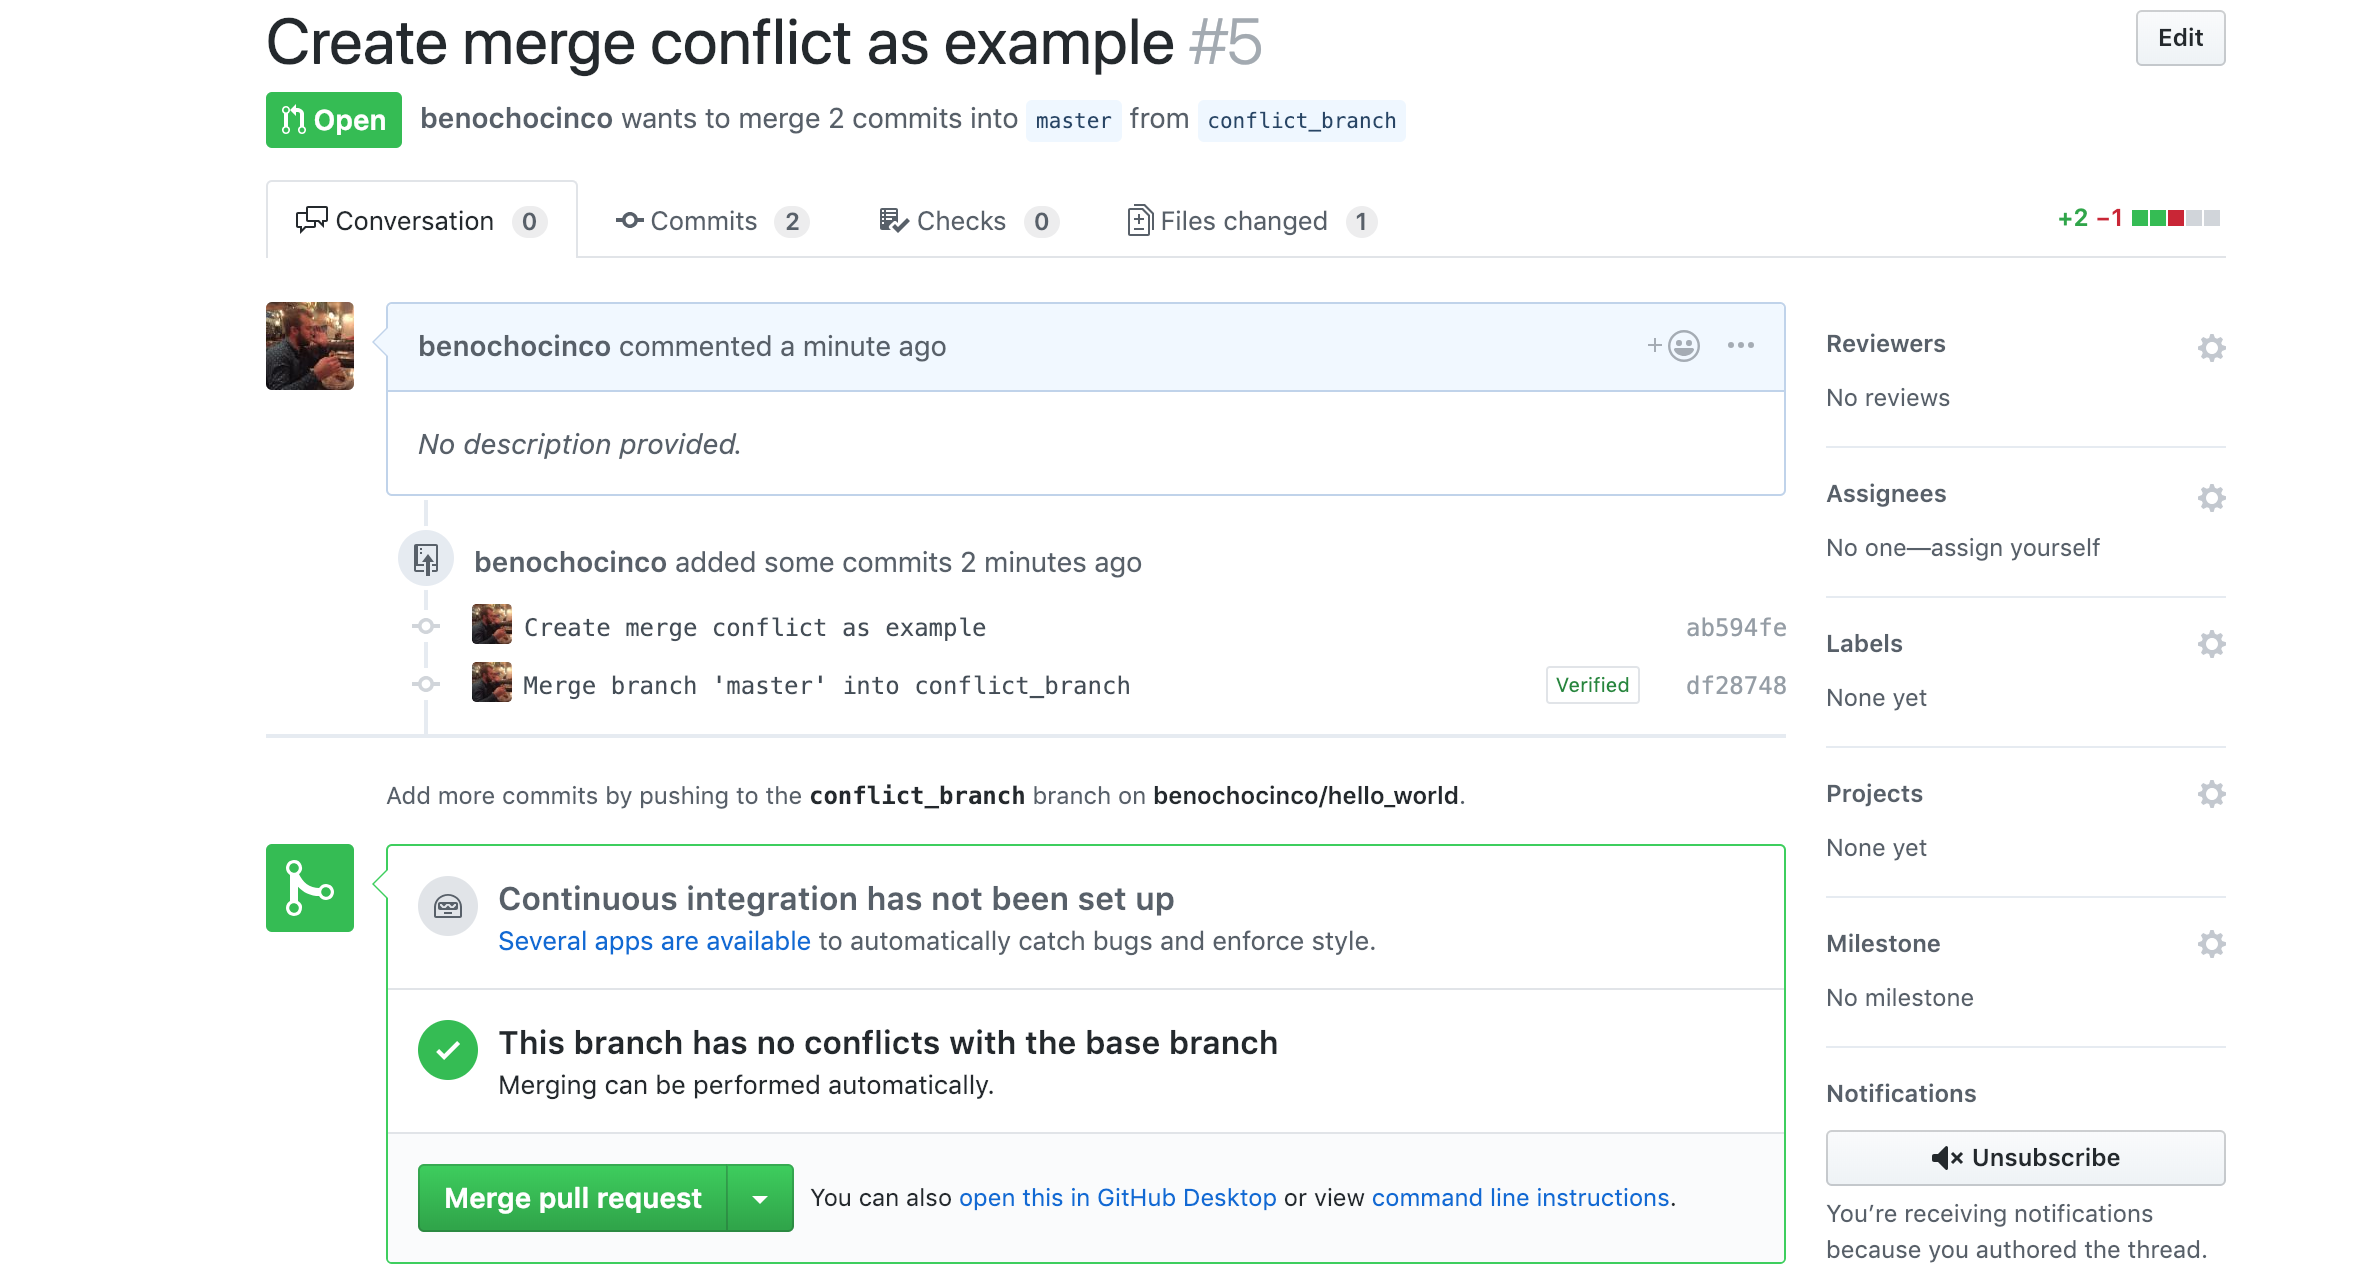
\includegraphics[width=.4\linewidth]{final_merge.png}
\end{subfigure}
\end{figure}
\end{frame}

\begin{frame}{Overview}
\begin{itemize}
    \item Step 1: Create your repository (i.e. codebase)
    \item Step 2: Clone your repository to your local computer
    \item Step 3: Create a branch
    \item Step 4: Make and commit changes to your branch
    \item Step 5: Open a pull request
    \item Step 5.5: Resolve merge conflicts (if you have any)
    \item Step 6: Merge your pull request
\end{itemize}
\begin{figure}
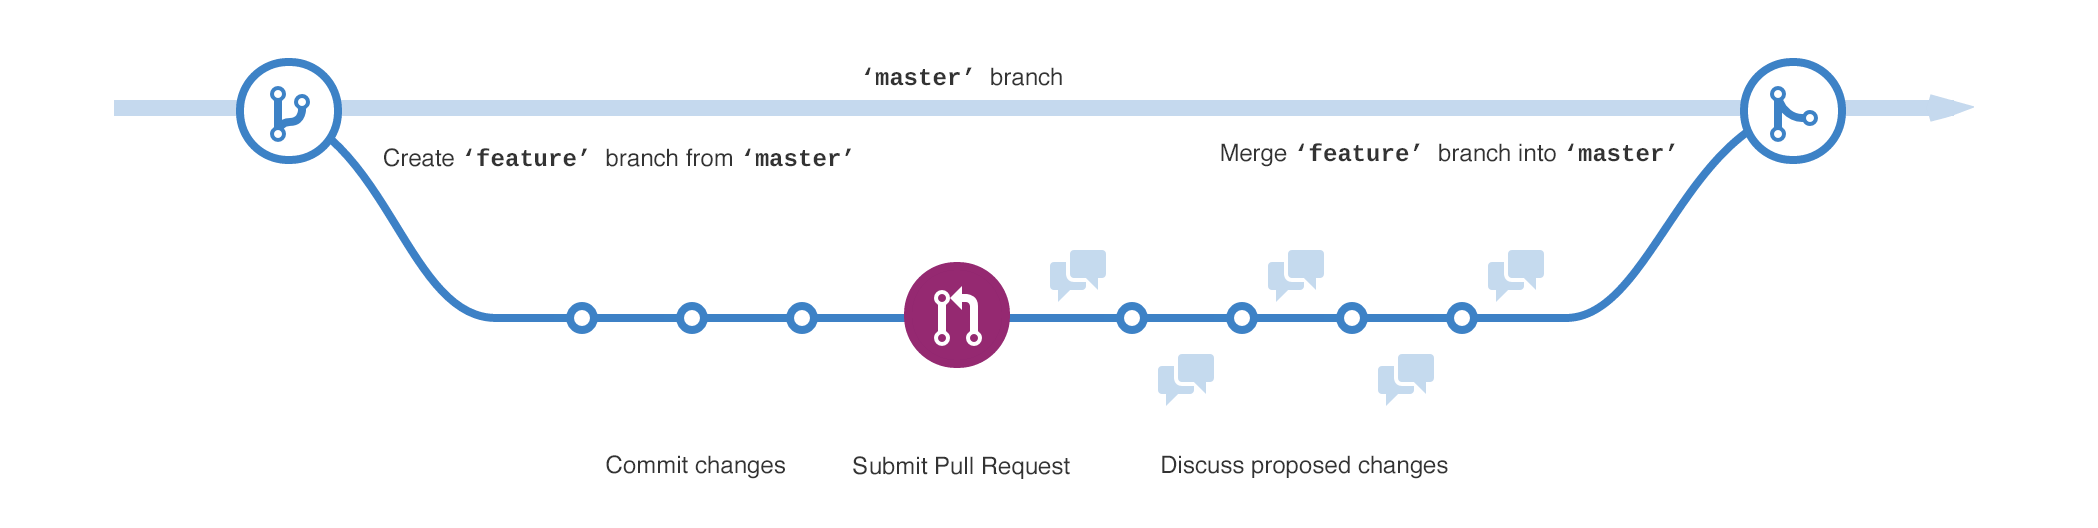
\includegraphics[width=10cm]{branching.png}
\caption{\label{fig:your-figure}GitHub Workflow}
\end{figure}
\end{frame}

\begin{frame}{Overview: Branching Process}
\begin{itemize}
    \item Step 1: Create new branch from \textit{master} for each new task
    \item Step 2: Make and commit your changes to the code until you have completed all of your sub-tasks for your modularized objective
    \item Step 3: Push the changes on your branch to GitHub
    \item Step 4: Open a pull request on github.com/your-username/your-repo 
    \item Step 5: Review all changes in codebase as a team and make sure there are no conflicts
    \item Step 6: Merge your pull request back into the master branch to update the codebase
\end{itemize}
\end{frame}

\begin{frame}{Now it's your turn!}
\begin{itemize}
    \item We will follow the GitHub tutorial at guides.github.com/activities/hello-world/ together!
        \begin{figure}
        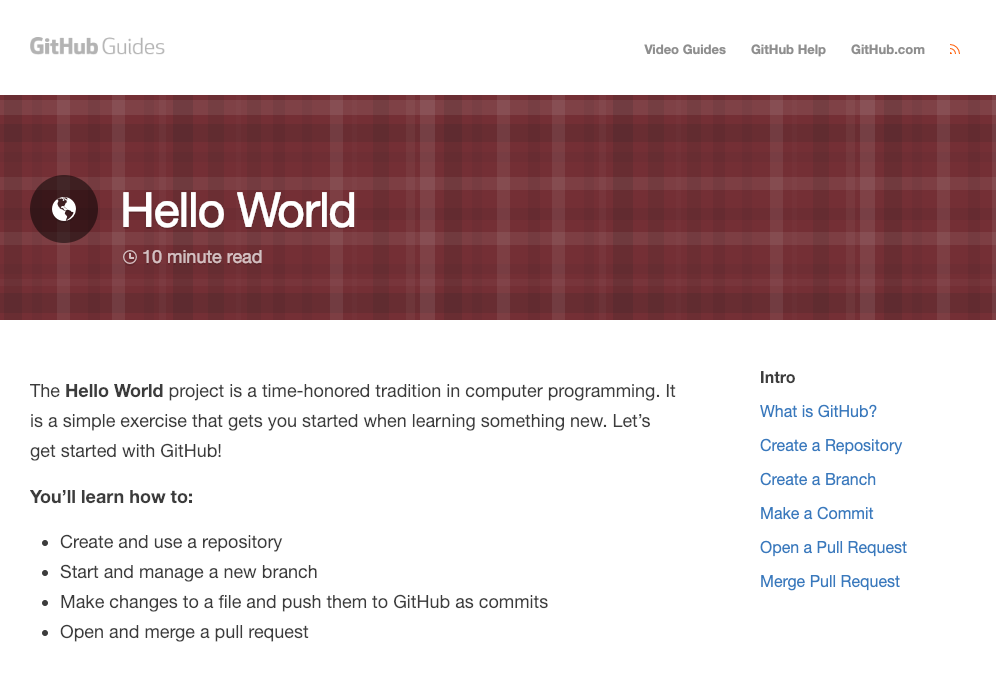
\includegraphics[width=4cm]{hello_world.png}
        \end{figure}
    \item Make sure you have set up your GitHub account and have downloaded and installed GitHub Desktop before starting
    \item \textit{Note}: You can use the command line like they do in the tutorial, but we will be working with GitHub Desktop
    \item Additional documentation on how to use GitHub Desktop can be found here: help.github.com/desktop/guides/
    \item Additional documentation on how the GitHub workflow works can be found here: guides.github.com/introduction/flow/
\end{itemize}
\end{frame}

\end{document}
